 \documentclass[12pt]{article}
 \usepackage[margin=1.2in,a4paper]{geometry}
 \usepackage[T1]{fontenc}
 \usepackage{textcomp}
 \usepackage{ragged2e}
 \usepackage{booktabs}
		  \usepackage{epltxfn} %expex footnotes
 \usepackage{bold-extra}
 \usepackage{fancyhdr}
 \usepackage{fontspec,xltxtra,xunicode}
 \usepackage[labelsep=period,font=small,labelfont=bf,small]{caption}
 \defaultfontfeatures{Mapping=tex-text}
 \setmainfont{Cambria}
 \newcommand{\HRule}{\rule{\linewidth}{0.5mm}}
 %\setromanfont[Mapping=tex-text]{Hoefler Text}
 %\setsansfont[Scale=MatchLowercase,Mapping=tex-text]{Gill Sans}
 %\setmonofont[Scale=MatchLowercase]{Andale Mono}
 

 \usepackage{Sanremo,lettrine}
 \renewcommand\LettrineFontHook{\Sanremofamily}
 
 % \usepackage[margin=.7in,nohead,right=1.5in]{geometry}
 \def\singlesidestandardsetup{
 	%\textwidth 6in
 	%\oddsidemargin 0in
 	%\evensidemargin 0in
 	%\topmargin -.5in
 	
 	%\textheight 9.5in
 	%\columnwidth \textwidth
 	\parindent 1em
 	%\parskip 8pt
 	\pagenumbering{roman}
 	\parindent 1em
 	\parskip 10pt
 	
 }
 \usepackage{marginnote}
 \xdef\marginnotetextwidth{\the\textwidth}
 
 \usepackage{wrapfig}
 %\newcommand{\longsquiggly}{\xymatrix@C=1.915em{{}\ar@{~>}[r]&{}}}

\fancypagestyle{plain}{%
	\fancyhf{} % clear all header and footer fields
	\fancyfoot[C]{\sffamily\fontsize{9pt}{9pt}\selectfont\thepage} % except the center
	\renewcommand{\headrulewidth}{0pt}
	\renewcommand{\footrulewidth}{0pt}}
\pagestyle{plain}

 
 \newcommand{\mcom}[1]
 {\marginpar{\raggedleft\raggedright\hspace{0pt}\linespread{0.9}\footnotesize{#1}}}
 \newcommand{\cb}[1]
 {\marginpar{\color{orange}\raggedleft\raggedright\hspace{0pt}\linespread{0.8}\footnotesize{#1}}}
 \newcommand{\hk}[1]
 {\marginpar{\color{purple}\raggedleft\raggedright\hspace{0pt}\linespread{0.8}\footnotesize{#1}}}

\newcommand{\mmp}[1]
{\marginpar{\color{green}\raggedleft\raggedright\hspace{0pt}\linespread{0.8}\footnotesize{#1}}}

 \newcommand{\note}[1]{{ }\mcom{Note}\textbf{#1}}
 
 \newcommand{\glem}[1]
 {\MakeUppercase{\scriptsize{\textbf{#1}}}}
 
 
 %%%%cancel margin notes
 \renewcommand{\mcom}[1]{}
 \renewcommand{\mmp}[1]{}
 \renewcommand{\cb}[1]{}
 \renewcommand{\hk}[1]{}
 
 \newcommand{\specialcell}[2][c]{%
 	\begin{tabular}[#1]{@{}c@{}}#2\end{tabular}}
 
 \makeatletter
 \def\@xfootnote[#1]{%
 	\protected@xdef\@thefnmark{#1}%
 	\@footnotemark\@footnotetext}
 \makeatother
 
 
 \newcommand{\xmark}{\ding{55}}
 
 
 
 \author{Josh}
 \date{\today}
 
 \usepackage{subfigure}
 \usepackage{amsthm}
 \usepackage[normalem]{ulem}
 \usepackage{amssymb}
 \usepackage{multirow}
 \usepackage{mathrsfs}
 \usepackage{pifont}
 \usepackage{mathtools}
 \usepackage{tikz}
 \usepackage{qtree}
 \usepackage{tikz-qtree}
 %\usepackage{tipa}
 \usetikzlibrary{decorations.pathreplacing}
 \usepackage{textcomp}
 \usepackage[normalem]{ulem}
 \usepackage{url}
 \usepackage[all]{xy}
 \usepackage{multicol}
 \usepackage{hanging}
 \usepackage{booktabs}
 \usepackage{setspace}
 \usetikzlibrary{shapes,backgrounds}
 \usepackage{geometry}
 
 
 
 \newtheorem{definition}{Definition}
 \newtheorem{theorem}{Theorem}
 
 
 \usepackage{enumerate}
  \usepackage{enumitem}
 %\usepackage{gb4e} \let\eachwordone=\sl
 \usepackage{expex}
 
 
 
 %\newcommand{\denote}[1]{\mbox{$[\![\mbox{#1}]\!]$}}
 \newcommand{\concat}{\mbox{$^\frown$}}
 \newcommand{\ph}{\varphi}
 \newcommand{\vsep}{\vspace{8pt}}
 \newcommand{\linesep}{\rule{6.5in}{.5pt}}
 \def\attop#1{\leavevmode\vtop{\strut\vskip-\baselineskip\vbox{#1}}}
 \newcommand{\denote}[1]{\mbox{$[\![\mbox{#1}]\!]$}}
 \newcommand{\exref}[1]{~(\ref{#1})}
 
 \newcounter{nextsec}
 \newcommand\nextsection{%
 	\setcounter{nextsec}{\thesection}%
 	\stepcounter{nextsec}%
 	\thenextsec%
 }
 \newcommand\nextsubsection{%
 	\setcounter{nextsec}{\expandafter\parsesub\thesubsection\relax}%
 	\stepcounter{nextsec}%
 	\thesection.\thenextsec%
 }
 \def\parsesub#1.#2\relax{#2}
 \def\parsesubsub#1.#2.#3\relax{#3}
 %\input{setup}
 
 %\singlesidestandardsetup
 
 %\parindent 1em
 
 %\input{psfig-scale}
 
 
 \newcommand{\verteq}{\rotatebox{90}{$\,=$}}
 \newcommand{\equalto}[2]{\underset{\scriptstyle\overset{\mkern4mu\verteq}{#2}}{#1}}
 
 
 \newcommand{\secsep}{\hrulefill}
 \renewcommand*{\marginfont}{\small}
 \usepackage{qtree}
 \qtreecenterfalse
 
 \renewcommand{\baselinestretch}{1} %% this is the linespacing
 
 \newcommand{\la}{\langle}
 \newcommand{\ra}{\rangle}
 \newcommand{\lamda}{\lambda}
 \usepackage{framed}

\begin{document}
\begin{center}
 	\thispagestyle{empty}
 	{\Large	\textsc{dissertation prospectus}}
\vfill
\HRule\vspace{.33cm}

\setcounter{page}{-1}
\textbf{{\huge The intersection of temporal \& modal interpretation:}\\
{\Large a view from Arnhem Land (northern Australia)}}\\\textit{working title}

\HRule
\vfill
{\small \textbf{Josh Phillips}}
\vfill
\textit{\textbf{Committee}}\\
\begin{tabular}{ll}
Claire Bowern (c.) & Yale U.\\
%Ashwini Deo (??) & Ohio State U.\\
Hadas Kotek & New York U.\\
%Lisa Matthewson (??) & U. of British Columbia\\
María Piñango & Yale U.\\
%Judith Tonnhauser (??) & Ohio State U.
\end{tabular}


\vspace*{.3in}{\color{gray} \textit{+ two vacancies}}

\vfill
\sc Department of Linguistics
	
	Yale University
	
	\today

	
\end{center}\newpage
\thispagestyle{empty}\tableofcontents\newpage
\section{Motivation}
\lettrine{D}{isplacement} --- a stated universal and distinctive feature of human language ---  permits us to make assertions that are embedded in different times, locations and possible worlds (\textit{e.g.} Hockett's `design features of human language' 1960:90). Linguistic work --- descriptive, pedagogical, theoretical --- has traditionally assumed a categorical distinction between subtypes of verbal inflection: \textit{viz.} the \textsc{temporal} and \textsc{modal} domains. Whether or not these basic claims are intended as heuristic, they quickly unravel upon close inquiry into cross-linguistic data; a challenge for linguistic theory, and one that a growing body of literature is identifying (\textit{e.g. }Condoravdi 2002, Laca 2008, Rullman \& Matthewson to appear \textit{i.a.}).% This will become clear in section \ref{phen} of this prospectus.

The \textbf{empirical focus} of the dissertation proposed here is the tense-mood-aspect (TMA) systems of a set of languages in the Arnhem Land linguistic area of Northern Australia. Arnhem Land is `linguistically dense' --- an area of close historic and contemporary contact between unrelated languages (see map in Figure \ref{map}). The verbal systems of many of these languages have evaded an adequate, unified account and exhibit various features that have been identified elsewhere as typologically rare (and certainly sharply diverge from better described Indo-European systems).

Consequently, given how resistant these data have been to description and analysis with existing linguistic apparatus, no theory neatly accounting for the inflectional range or making predictive generalisations; a better understanding of these systems will help us to nuance the way we think about categories like `tense' and `modality' --- a theory of temporomodal displacement. The potential \textbf{theoretical contribution} of this dissertation, then, bears broadly on \textit{intensionality}: our notional categories of tense, mood, modality, aspect, evidentiality, conditionals \textit{etc.} Further, as will be shown in §2, the role of pragmatics/information structure and their interactions with semantics are crucial for understanding how these categories are expressed and interpreted: how intensional meanings are generated, how communication permits for the displacement of times and worlds.

% a theoretical framework that can provide a (compositional) analysis of the data, whether small or large changes to existing work or a new proposal remains to be seen. This is relevant for anyone who works on anything intensional, including modality, tense, aspect, evidentiality, conditionals (counterfactuals, unconditionals, etc), to name a few


\begin{figure}
\centering\caption{Traditional language communities in Northern Australia (Horton 1996).\\\textbf{Inset. }Northeast Arnhem land (colourised from Wilkinson 1991:2). Yellow shading indicates the \textit{Yolŋu Wäŋa} (homeland). Brown and green circles indicate the contemporary distribution of Yolŋu languages investigated. Purple circling indicates the neighbouring Maningrida language family. Kriol is spoken in all communities in the southern half of this map.}	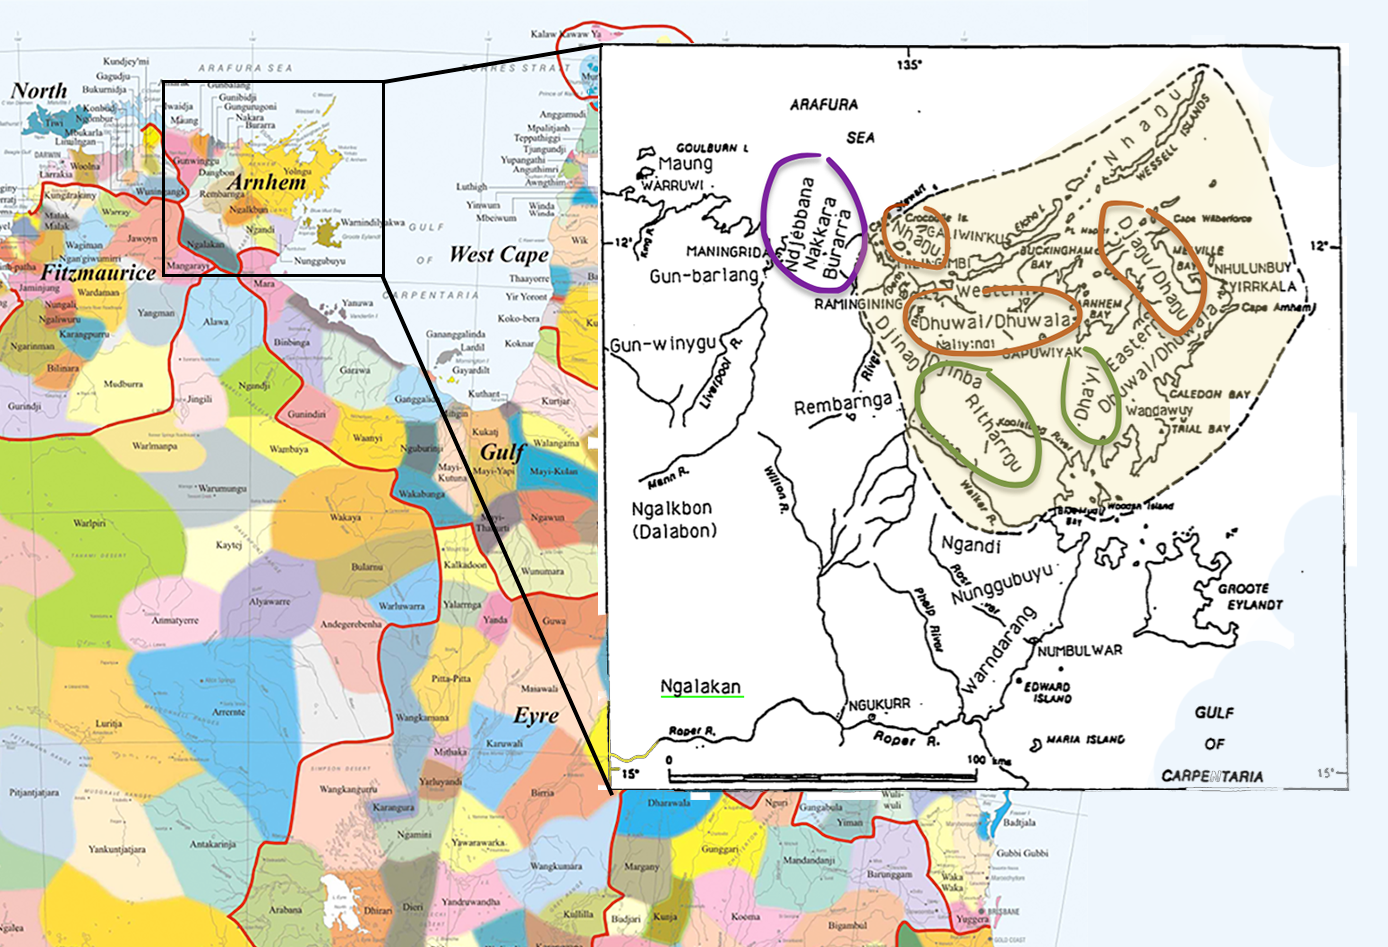
\includegraphics[width=0.8\textwidth]{AustralianLangsCropped.png}\label{map}
\end{figure}


Additionally, in this work I seek to consider the contribution of studying \textbf{language change} (specifically meaning change) to a better understanding of the cognitive apparatus that permits for the interpretation of temporomodal devices (\textit{sc. `what is it that speakers are doing in order to `displace' discourse?}). A starting point in the assumption that `diachronically consecutive grammars are not characterised by radical discontinuities or unpredictable leaps, but that change consists of gradual discrete steps constrained by properties of grammar' (Deo 2006: 5). By hypothesis, then, the investigation of these `steps' between subsequent stages of a grammar with respect to its verbal semantics--and the inference of `constraints' on these changes--represent a significant potential source of insight into the linguistic expression and evaluation of event structure, time and possibility.
\hk{Add a paragraph about what you expect the main contributions of your work to be. I imagine it's something like:  
• a description of several understudied languages, specifically with respect to their TMA systems. This is important for anyone working on these phenomena.\\• a theoretical framework that can provide a (compositional) analysis of the data, whether small or large changes to existing work or a new proposal remains to be seen. This is relevant for anyone who works on anything intensional, including modality, tense, aspect, evidentiality, conditionals (counterfactuals, unconditionals, etc), to name a few.\\• a diachronic perspective. This one you actually do a good job or spelling out.}
%(or perhaps amphichronic, in the sense of Kiparsky 2006) approaches to linguistics represent an fount of insight into the relationship between 

This prospectus is organised into four sections: this statement of motivation, followed by \textbf{§\ref{phen}}, which introduces examples of particular phenomena in Arnhem Land languages, analyses of which form the focus of the dissertation. The subsequent section \textbf{(§\ref{lit})} seeks to identify and situate this work within the broader scholarship of the semantics and interpretation of verbal inflectional categories. The final sections draft a chapter structure and schedule to completion of the proposed dissertation \textbf{(§4)}. Additional data is provided in appendix.



\section{Tense-Mood interactions in Arnhem Land}\label{phen}

As indicated above, data from Australia's 400+ indigenous languages have not been explicitly accounted for in the elaboration of formal semantic work. Temporal and modal phenomena in these languages appear to pose some problems for our models. The proposed dissertation seeks to marshal synchronic and diachronic data to nuance our understanding of the interpretation of temporal and modal operators. \textbf{§\ref{rop}} summarises a diachronically-informed account of the emergence of modal meaning from a temporal frame adverbial in Australian~Kriol~\texttt{[rop]}, a contact language borne of early Twentieth Century frontier expansion in Southeastern Arnhem Land, varieties of which are now spoken across many communities in northern Australia (see Harris 1986, Sandefur 1986).

\textbf{§\ref{yol}} provides a comparative overview of the verbal paradigms of some Yolŋu languages, which are problematic for standard model-theoretic conceptualisations of tense and modal semantics. These phenomena are examples of the work that will be developed through the proposed dissertation.\mcom{`examples' --- too mysterious?} Data and existing descriptive and analytic work are described in this section in addition to a preliminary analysis.

While Kriol and Yolŋu varieties are not `genetic' relatives of one another, they are neighbouring languages (with some southern Yolŋu varieties in sustained contact situations with Kriol). As we will see, both provide clear examples of phenomena that present similar analytic challenges to semantic theory --- the well-understood categories which form the basis of the theory fail in these cases to predict changes or capture generalisations that adequately describe phenomena integral to the meaning of the inflectional paradigms of these varieties.\hk{reword final sentence?}
\hk{\textbf{General comment 1:} okay so really what I'm missing at this point is detail. What specifically are you looking at? Is there a concise way to explain what challenges the data pose (even just a couple of examples) so your readers can get a sense of what you're going to show and do? }
\subsection{\textsc{\textbf{Kriol}}. Temporomodal polysemy and the emergence of \\\textsc{appr}ehensional marking}\label{rop}

Australian Kriol is a contact language spoken through many communities in Northern Australia, including much of southern Arnhem Land. The Ngukurr variety is generally considered to be the `birthplace' of this language, a result of radical language contact between English-based pidgins and a number of Arnhemland substrates in the early twentieth century.


Recent work has shown the apparent recruitment of a temporal frame adverbial (TFA) \textit{bambai} $<$ `by-and-by' (a lexical item present in many Pacific contact languages) as a marker of so-called \textsc{apprehensional} modality (\textit{see} Angelo \& Schultze-Berndt 2016; Phillips forthcoming.) Apprehensionals are a grammatical category widely represented in Australian (in addition to Austronesian, Amazonian etc.) languages. In one of the only published works dedicated to a treatment of apprehensionals, Lichtenberk (1995) describes these markers as dually encoding (a) an assertion of the possibile instantion of their prejacent (his ``epistemic downtoning'') and (b) information about negative speaker affect vis-à-vis their prejacent. The sentence pair in (\nextx) shows these two possible uses (\textit{viz.} temporal or modal) of \textit{bambai}. Both sentences are possible responses to an invitation.

\pex\textbf{Context:} I've invited a friend around to join us for dinner. They reply:	
\a\begingl\deftagex{pres}\deftaglabel{seq}
\gla yuwai! \textbf{bambai} ai gaman jeya!//
\glb yes! \textit{\textbf{bambai}} 1s come there//
\glft `Yeah! I'll be right there!'//
\endgl
\a\deftaglabel{m}\begingl\deftaglabel{appr}
\gla najing, im rait! \textbf{bambai} ai gaan binijim main wek!//
\glb no 3s okay \textit{\textbf{bambai}} 1s \textsc{neg.mod} finish 1s work//
\glft`No, that's okay! (If I did,) I mightn't (be able to) finish my work!'\hfill(GT~13072017)//
\endgl
	\xe

In (a), \textit{bambai} simply displaces the reference time of the prejacent slightly forward; the speaker has undertaken to join for dinner in the near-immediate future of speech time. Conversely, the apprehensional use is shown in (b); here, the speaker asserts that, in the event that they join for dinner, they may fail to complete their work (a negative outcome).

Similarly, as shown in the sentence pair (\nextx), this apprehensional meaning also appears in past irrealis (i.e. counterfactual) contexts.

\pex\a\begingl
\gla ai\textdblhyphen{}bin wotji muvi en \textbf{\textit{bambai}} aibin silip$\sim$silip//
\glb 1s\textdblhyphen\textsc{pst} watch film and \textit{\textbf{bambai}} 1s\textdblhyphen\textsc{pst} sleep$\sim$\textsc{red}//
\glft`I watched a film last night, \textbf{then shortly afterwards}, fell asleep'//\endgl

\a \deftagex{sjv}\deftaglabel{A}\begingl
\gla ai\textdblhyphen{}bin dringgi kofi nairram \textbf{bambai} ai bina silip$\sim$silip-bat la wek//
\glb 1s\textdblhyphen{\sc pst} drink coffee night \textit{\textbf{bambai}} 1s {\sc pst:irr} sleep{\sc$\sim$red-ipfv} {\sc loc} work//
\glft`I had coffee last night, \textbf{otherwise} I may've fallen asleep at work' \hspace*{\fill}(AJ~23022017)//%\\\textsc{prejacent$_q$:} `I would've fallen asleep at work'//
\endgl
\xe

The apprehensional reading shown in both (b) examples above appears to have emerged out of what I term the `subsequential' reading of \textit{bambai}, one that is shared by \textit{bambai}'s many cognates in related Pacific contact varieties and the English etymon (Harris 1986: 210).\hk{provide an example of this from another PCV}

In table \ref{triggers} below, I list the contexts in which apprehensional readings of Kriol \textit{bambai} appears to emerge. Notably all of these can be understood as triggering an interpretation of an utterance in \textbf{nonfactual speaker mood}. That is, these clauses express `a hypothetical assumption...or otherwise some question about the actual truth of the clause' (Roberts 1989: 686-7).

\footnotetext[1]{This does not entail the claim that these operators are in any way semantic primitives.}
\footnotetext[2]{ Except where noted, these data were collected by the author in the field in 2016 and 2017.}
\footnotetext[3]{This example due to Dickson (2015:168 [KM~20130508]).}

\begin{table}[h]\caption[Semantic operators]{Semantic operators\footnotemark{} that appear give rise to modalised readings of \textit{bambai}.\footnotemark}\label{triggers}\small\centering
	\begin{tabular}{lll}\toprule
		\glem{Gloss} & \textbf{Morph} & \textbf{\textit{Example}} \\\midrule\midrule
		\textsc{irrealis} & \textit{garra} & \specialcell[l@]{\textit{ai\textbf{rra} dringgi kofi \textbf{bambai} mi gurrumuk}\\`I'll have a coffee or I might fall asleep'}\\\midrule
		\textsc{prohibitive} & \textit{kaan} & \specialcell[l@]{\textit{ai \textbf{kaan} dringgi kofi \textbf{bambai} mi nomo silip}\\`I won't have a coffee or I mightn't sleep'}\\\midrule
		\textsc{counterfactual} & $\underset{\textsc{pst:irr}}{bina}$ & \specialcell[l@]{\textit{ai \textbf{bina} dringgi kofi nairram \textbf{bambai} aibina silip}\\`I had a coffee last night or I might've fallen asleep'}\\\midrule
		\textsc{imperative} & $\varnothing$ &\specialcell[l@]{\textit{yumo jidan wanpleis \textbf{bambai} mela nogud\footnotemark}\\`Youse sit still or we might get cross'}\\\midrule
		\textsc{prohibitive} &  $\underset{\textsc{impr}\!\!}{\varnothing}$[\textit{nomo}] & \specialcell[l@]{\textit{\textbf{nomo} krosim det riba, \textbf{bambai} yu flodawei}\\`Don't cross the river or you could be swept away!'}\\\midrule
		\textsc{generic} & $\varnothing$ &\specialcell{\textit{im gud ba stap wen yu confyus, \textbf{bambai} yu ardim yu hed}\\`It's best to stop when you're confused or you'll get a headache'}\\\midrule
		\textsc{negative} & $\underset{\textsc{gen}}{\varnothing}$[\textit{nomo}] & \specialcell{\textit{ai \textbf{nomo} dringgi kofi enimo \textbf{bambai} mi fil nogud}\\`I don't drink coffee anymore or I feel unwell'}\\\midrule\midrule
		{\sc conditional}&\textit{if}&\specialcell[]{\textit{\textbf{if} ai dringgi kofi \textbf{bambai} ai kaan silip}\\`If I have coffee, then I mightn't sleep'}\\\bottomrule
		
		
	\end{tabular}

\end{table}

\subsubsection{A unified semantics for \textit{bambai}}

In (\nextx), then, I propose a denotation that goes part of the way to providing a unified treatment of these two uses. It is based on the insight that temporal frame adverbials of the \textit{bambai}-type, appear to induce an expectation of soon-ness (here `subsequentiality') on the instantiation time of their prejacent. This subsequentiality relation can be understood to represent the `kernel' of meaning at the heart of both readings of \textit{bambai.}



\pex\a\deftagex{ssqIsem}\textbf{Subsequential Instantiation} (intensionalised)\\$\text{{\sc subseqInst}}(P,t,w)\leftrightarrow\exists t^\prime:t^\prime\succ{}t\wedge\text P(t^\prime)(w)\wedge\mu(t,t^\prime)\leq s_c$


\textsl{In words:} a subsequentiality relation {\sc subseqInst} holds between a predicate $P$, reference time $t$ and reference world $w$ iff the $P$ holds in $w$ at some time $t^\prime$ in the future of $t$.\\Additionally they assert that the temporal distance $\mu(t,t^\prime)$ between reference and event time must be below some contextually provided standard of `soon-ness' $s_c$. %modulo vagueness??


\a $\denote{bambai}^{t,w}\!\underset{\text{def}}{=}\lambda f\lambda g\lambda P.\exists w\,^\prime\in\boldsymbol{Best}(f,g,t,w)\wedge\text{{\sc subseqInst}}(P,t,w\,^\prime)$

\textsl{In words:} \textit{bambai} asserts that there exists some world $w^\prime$ in a set of worlds that are optimal with respect to a contextually-determined modal base $f$ and ordering source $g$ in the reference context $\la t,w\ra$. It additionally asserts that the {\sc subsequential instantiation} relation holds between that world $w^\prime$, the prejacent $P$, and the reference time $t$.
\xe


My second qualifying paper proposed that that temporal frame (sc. `subsequential') uses of \textit{bambai} differ from apprehensional uses in terms of the \textsc{conversational background} $f,g$ that is selected (cf. Kratzer 1981 a.o). These conversational backgrounds must be retrieved from context, linguistic or nonlinguistic.

With the entry in (\lastx), we can formalise the intuition that, when predicating into an unsettled timeline\hk{def unsettled} \denote{bambai $p$} represents an epistemic claim. We model this by claiming that under these conversational backgrounds, \textit{bambai} has selected an \textit{epistemic} modal base $f_{\text{epist}}$ and a stereotypical ordering source. These conversational backgrounds are formalised in (\nextx), adapting liberally from Kratzer (2012: 37,39-40 a.o.)%\mcom{It is essential to find some way of intersecting the (negation of???) the antecedent with the modal base otherwise this is literally just $\lozenge$. What we have here however does give \denote{bambai $P$}, we also need $\denote{Q bambai P}$}
\small
\pex\a\deftagex{epistmod}$\bigcap f_{\text{epist}}(w)(t)=\{w^\prime\mid w^\prime\text{ is compatible with what \textsc{Speaker} knows in $w$ at $t$\}}$
\a $g_{\text{s'typ}}(w)=\{p\mid p\text{ will hold in the `normal' course of events in }w\}$.
\a$g(w)$ then induces an ordering $\leq_{g(w)}$ on the modal base:

\hspace{-.45cm}$$\forall w^\prime\!,w^{\prime\prime}\!\in\bigcap f_{\text{epist}}(w)(t):w^\prime\!\boldsymbol{\leq_{g(w)}}\!\!w^{\prime\prime}\leftrightarrow\{p:p\in g(w)\wedge ^{\prime\prime}\in p\}\subseteq\{p:p\in g(w)\wedge w^\prime\in p\}$$\\
\hspace{.3cm}
\textsc{In words:} for any worlds $w^\prime$ and $w^{\prime\prime\!}$, $w^\prime$ is `at least as close to an ideal' as $w^{\prime\prime}$ with respect to $g_{\text{s'typ}}(w)$ (\textit{i.e.} it is at least as close to the `normal course of events') if all the propositions of $g(w)$ true in $w^{\prime\prime}$ are also true in $w^\prime\!$.
\a \textbf{\textit{Best}}$(f_{\text{epist}},g_{\text{s'typ}},t,w)$ then returns just that subset of worlds that are both consistent with what the Speaker knows at $t$ in $w$ that are closest to the normal unfolding course of events in $w$.
\xe\hk{\textbf{Gen. comment 2} 

Reorganization suggestion -- (a) slow down the description of data. Maybe add the Eve example to strengthen the notion of "contextually soon", which sort of comes out of no where. 

(b) clarify whether you think there's one underlying use or two uses of bambai, and how that relates to the previous work on bambai. 

(c) briefly introduce the framework you're going to use to model bambai. State at the outset that it's a modal framework based on work by Kratzer. Define relevant notions (modal base, ordering source) with simple examples 

(d) walk the reader through your logic as you construct your proposal. 

(e) don't forget to define things as you go (e.g. unsettled timelines). Consider showing short examples of how your analysis works, so it's not all vague and theoretical. }


\normalsize
The so-called subsequential TFA use of \textit{bambai}, then, is maintained when the discourse context fails to R-implicate that the Speaker is making a non-modalised claim (cf. Grice's Quality$_2$)\footnote{\textit{I.e.} \textit{`Do not say that for which you lack adequate evidence'} (Grice 1991: 27, a.o.)}. That is, in contexts where the speaker can be understood to have access to the requisite facts to make an assertion about a subsequentiality relation between time and event, then the `actuality' of this claim is entailed.

In these cases the intensional contribution of \textit{bambai} can be captured by claiming that it quantifies (trivially) over a \textit{metaphysical} modal base and a \textit{totally realistic} ordering source (adapted partially from Kratzer 2012.)\footnote{This component of the analysis has additionally benefited greatly from Deo who makes use of similar formalism in her treatment of present tense semantics (2017).}

\pex
\a\deftagex{metamod}$\bigcap f_{\text{meta}}(w)(t)=\{w^\prime\mid w^\prime\simeq_t w\}$
\a $ g_{\text{real}}(w)=\{w\}$
\a \textbf{\textit{Best}}$(f_{\text{meta}},g_{\text{real}},t,w)$ then simply returns a set of worlds which are historical alternatives to $w$ at $t$ (\textit{i.e.} those that best comply with all the propositions that uniquely characterise $w$).
\xe


\subsubsection{Selecting a conversational background}
Ultimately, the interpretation of \textit{bambai} must be anaphoric on discourse context, apprehensional readings restricted to propositions made in the `nonfactual speaker mood' (cf. Roberts 1989). This can be understood as the operationalisation of the pragmatic principle described in (\nextx).

\pex\textsc{\textbf{The omniscience restriction.}} It is notable that, in the apprehensional cases presented above---those where predication into an unsettled timeline has been triggered by one of the operators presented in Table \ref{triggers} above--- modalisation with respect to a non-settled property cannot reasonably select for the set of conversational backgrounds presented in (\lastx). Such an operation would require the participants to be able to retrieve all propositions that are true in and characteristic of worlds with respect to a vantage point in the future or to be able to calculate all the ramifying consequences of eventualities that might have (but ultimately failed to) obtained in the past. This condition allows us to unify the modalised and non-modalised readings of \textit{bambai}.
\xe

		\hk{\textbf{Gen comment 4}
		
		Rewrite and reframe this last paragraph. It could be its own section, roughly here (the other part I think should move up), introducing a problematic example and sketching a solution. If you spend an entire section spelling out a theory, you should not end that section by saying that what you did up until now doesn't work. It's fine to say that additional data will lead to a refinement of the theory or to the adoption of a dynamic framework to work within, to cash out insights that a static approach doesn't give you (and you will probably need to explain what static/dynamic mean here) -- but it should be clear that it's an addition/refinement of what you've done, not replacing it (or, again, why did you make us read all this wrong stuff?) 
		
		In other word: we should get the strongest and clearest arguments and a good, working, final result. We don't necessarily need to get the whole story of how you discovered this solution and all the steps that didn't work along the way. 
		}
The emergence of new data shows that the omniscience restriction as formulated in (\lastx) is too strong by itself; it fails to predict the \textit{felicity} of the subsequential reading in (\getfullref{pres.seq}). The interpretation of \textit{bambai} then seems to provide evidence for the necessity of considering both extralinguistic factors (\textit{i.e.} world knowledge and notions of the \textit{common ground} (see Stalnaker 1979) and intersentential dependencies and speaker mood (i.e. discourse structuring, \textit{e.g.} Kamp 1981; Heim 1982; Roberts 1989, 1998.) The insights from the information structure and dynamic semantics literatures can provide a vital framework to help us to understand the heuristic devices which allow speakers to identify an antecedent to \textit{bambai} (by which to restrict the quantificational domain as formalised in (\getref{epistmod}-\getref{metamod}) above) and to disambiguate these readings. These issues will be discussed in detail in Chapter 4 of the dissertation.

\subsubsection{A diachronic perspective}
In addition to the synchronic analysis described above, \textit{bambai} provides a case study of the clear emergence of modal meaning from an erstwhile temporal adverbial in particular supporting contexts. I suggest that a discussion of the apparent semanticisation of apprehensional readings can be best explained in terms of invited inference theory (\textit{e.g.} Traugott 1989, Eckardt 2006, Deo 2015a). 

In (\nextx) below, the translation provided elucidates the capacity of the temporal properties of \textit{bambai} \textit{qua} sequential TFA to implicate additional nontemporal properties of the relation between the clauses it links. Via pragmatic strengthening (\textit{sc.} the `invitation' of a {\em post hoc ergo propter hoc} inference), \textit{bambai} can be understood to assert that there exists some type of logical (\textit{e.g.} etiological) relation between the predicate contained in the first proposition and the negative eventuality described in \textit{bambai}'s prejacent: the second clause.\footnote{There is an extensive literature investigating the pragmatics of clausal connection/concatenation \textit{e.g.} Schmerling 1979, Stukker \& Sanders 2012 a.o. (for English).}

\pex[everylabel=\sc]\label{flodawei} \textbf{Context:} It's the wet season and the Wilton River crossing has flooded.
\a\begingl
\gla nomo krosim det riba!//
\glb {\sc neg} cross.{\sc tr} the river//
\endgl
\a 	\begingl\gla \textcolor{gray}{ba wani?}//
\glb \textcolor{gray}{why?}//
\endgl
\a[label=A]\begingl\gla bambai yu flodawei!//
\glb \textbf{\textit{bambai}} 2s float~away//
\glft`Don't cross the river \textcolor{gray}{[...why (not)?...]} Then you'd be swept away!'\hspace*{\fill}(GT~16032017)//\endgl\xe

The conventionalisation of \textit{bambai}'s connective syntax and its frequent embedding underneath (alternatively, its semantic `subordination to' in the parlance of Roberts 1989) warnings, prohibitives (\textit{e.g. }\lastx\textsc{a}) and predicates of fearing, appear to be a likely source of the semanticisation of the apprehensional reading.

In addition to these insights, however, the unified denotation that is proposed above also suggests the existence of a conceptual link between (relative) future marking and epistemic modalities, in keeping with observations made elsewhere on the semantics of the future tense (\textit{e.g.} Copley 2001, Palffy-Muhoray 2016 \textit{i.a.}, see also Bybee \textit{et al. 1994:247\textit{ff}}). The demonstration of this possible meaning change trajectory likely represents \textit{per se} additional support for the conceptual unity of futurity marking and epistemic modalities. This appears to be a function of the conventionalisation of speaker-based inferences that humans' predication into the future is necessarily specultative and informed by their own understanding of their world and observations of relations between possible situations.

\subsection{\textsc{\textbf{Yolŋu Matha}}. Meaning and change in the verbal inflectional paradigm}\label{yol}

Yolŋu Matha is a language family spoken in northeastern Arnhem Land. Internal classification and subgrouping has been somewhat controversial, but most treatments understand the family as containing six languages with thirty or so `clan-lects' distributed between them. For the purposes of this prospectus, I will make reference to the closely related Western varieties of Djambarrpuyŋu (\texttt{[djr]} Dhuwal) and Gupapuyŋu (\texttt{[guf]} Dhuwala), slightly further afield Wangurri (\texttt{[dhg]} Dhaŋu) and Southern variety Ritharrŋu \texttt{[rit]}, the varieties for which there is the most significant amount of presently available documentation.

The verbal inflectional paradigms of contemporary Yolŋu languages can be reconstructed to proto-Yolŋu (\textit{e.g.} Bowern 2009). Notwithstanding this demonstrated cognacy, there is significant cross-linguistic variation reported in the distributions and `meanings' associated with each of the four inflectional categories that appear on verbs in these languages (glossed throughout this prospectus as capital roman numerals \textbf{I\textasciitilde{}IV}). Where eastern and southern language varieties are described as having `basic tense categories' that are `semantically straightforward' (\textit{e.g.} Heath 1980 on Ritharrŋu:74\textit{ff}), an adequate treatment of the morphosemantics of tense marking in the related Yolŋu languages spoken in western Arnhem Land appears to be much more elusive notwithstanding the nuanced and detailed descriptions in Wilkinson 1991 and McLellan 1992. Consider to begin, the minimal pair in (\nextx) below.

\pex<wangI>\label{wangI} \textbf{Apparent insensitivity of verbal morphology to tense distinction in Wangurri}
\a\begingl
\glpreamble \textsc{Nonfuture use}//
\gla nhän \textbf{gayŋa} ŋirrima-ḻi \textbf{ŋarra}//
\glb 3s \textsc{ipfv} home-\textsc{all} go.\textbf{I}//
\glft`they went/were going home' (\textsc{pst}) \textbf{\textit{or}} `they're going home' (\textsc{pres})//
\endgl 
\a\begingl \glpreamble\textsc{Future use}//
\gla nhän \textbf{ŋarru} ŋirrima-ḻi \textbf{ŋarra}//
\glb 3s \textsc{irr} home-\textsc{all} go.\textbf{I}//
\glft`they will/should/must go home'\hfill(\texttt{[dhg]} McLellan 1992:154)//
\endgl
\xe

In (\lastx), the verbal inflection alone (glossed here as \textbf{I}) fails to disambiguate tense altogether: it provides no information on whether the event described (\textit{viz.} it \textsc{go} home) obtains in an interval preceding, subsequent to or overlapping with the speech time. This information must be provided by context or by aspectual/modal auxiliaries.

Additionally, Western Yolŋu varieties exhibit a phenomenon which Comrie refers to as `cyclic tense' --- an ostensibly areal feature and crosslinguistic rarity that it shares with the neighbouring, unrelated Maningrida language family.\footnote{Little typological work has been done on cyclical and metrical tense systems. Nevertheless, in this important cross-linguistic survey of tense systems, Comrie identifies these systems as uncommon, pointing only to Burarra (\texttt{[bvr]} Maningrida: W Arnhem), and perhaps Kisksht (\texttt{[wac]} Chinookan: Columbia River) and Bamiléké (\texttt{[ybb]} Niger-Congo: Cameroon). Bybee \textit{et al.} (1994:104) also point to a particle in Palantla Chinantec (\texttt{[cpa]} Oto-Manguean: Oaxaca) that appears to refer, discontinuously, to events completed the previous day \textit{or} immediately prior to utterance time (\textit{i.e.} `earlier today' reference is out and receives its own dedicated prefix (citing Merrifield 1968:25).)}
\textit{Cyclic tense} refers to a phenomenon where tenses have `discontinuous time reference', ostensibly arising from `the combination of two oppositions, one an absolute cut-off point between today and earlier than today, the other between recent and remote within each of these two time frames' (1985:89). Claims about the properties of \textit{cyclic tense} systems are discussed in more detail in §\ref{cyctns} below. The examples that follow in (\nextx) demonstrate this discontinuity and grammatical metricality. \textbf{Cyclicity} is manifested in the fact that all threes sentences predicate into the past; the event in (a), temporally intermediate to the other two is inflected with the primary verb form whereas those in (b,c) are inflected in the tertiary form. \textbf{Metricality} is best shown in the difference between (a) and (c): the seeing event in (a) is framed as a recent event whereas the growing event in (c) is framed as remote. These are schematised in Figure \ref{funnytense}.


\pex \textbf{Cyclicity and metricality in Djambarrpuyŋu}
\a\deftagex{pasts}\begingl\glpreamble\textsc{Recent past with \textbf{I}}//
\gla yo barpuru-ny ŋarra ŋaɲa nhä-\textbf{ma}-ny (*nhäŋal)//
\glb	yes, yesterday{\sc-prom} 1s 3s{\sc.acc} see-\textbf{I/*III}-{\sc prom}//
	\glft`Yes, I saw him yesterday'\footnotemark//\endgl
\a\begingl\glpreamble\textsc{Today past with \textbf{III}}//
\gla ŋe gäthur ŋarra ŋanya nhä-\textbf{ŋal} goḏarr dhiyal//
\glb	yes, today 1s 3s{\sc.acc} see-\textbf{III} morning {\sc prox-loc}//
	\glft`Yes, I saw him here this morning'//\endgl
	\a\begingl\glpreamble\textsc{Distant past with \textbf{III}}//
	\gla maarrma ga-\textbf{n} malwan-dja dhära-\textbf{n} yindi maṉḏa-ɲ//
	\glb two {\sc ipfv-\textbf{III}} Hibiscus-{\sc prom} stand-\textbf{III} big 3d-{\sc prom}//
	\glft`Two big Hibiscus flowers were growing there' (at some place in the speaker's youth)\hfill(Wilkinson 1991: 339)//
	\endgl
\xe
\footnotetext{Note that, as McLellan points out of the  phonologically-identical Wangurri cognate, \textit{barpuru}, while translated as `yesterday', can mean `the time of some ``recent specific event''' (1992:155). Cognates in related languages do have a strict `day before today' reading (Claire Bowern, pers. comm.)}


\begin{figure}[h]\centering\caption{Temporal expression in Western Yolŋu dialects, demonstrating two descriptive phenomena: (a) cyclicity --- the interspersion/discontinuity of \textbf{I} and \textbf{III} forms and (b) metricality --- the (subjective) division of the past domain between these two forms.\\$\lfloor{\sl today}$ is the beginning of the priveleged interval {\sl today}. $\boldsymbol{t*}$ is utterance time}\label{funnytense}
	\begin{tikzpicture}
	% draw horizontal line   
	\draw[<->, line width=.5mm] (0,0) -- (10,0);
		
		%draw rex
	\shade[left color=blue!10!white, right color=green!10!white] (0,0.02) rectangle (4.8,1.5);
%	\fill[green!10!white] (2.5,0.02) rectangle (4.8,1.5);
	\fill[blue!10!white] (4.8,0.02) rectangle (6.8,1.5);
	\fill[green!10!white] (6.8,0.02) rectangle (9.5,1.5);
	\fill[orange!10!white] (9.5,0.02) rectangle (10,1.5);
	
	% draw nodes
	\draw (1.25,0) node[below=3pt] {\textbf{}} node[above=10pt] {\textsc{\textbf{III}}};
	\draw (3.675,0) node[below=3pt] {\textbf{}} node[above=10pt] {\textbf{I}};
	\draw (5,0)   node[circle,fill,label=below:$\lfloor{\sl today}$] {} node[below=3pt] {\textbf{}} node[above=3pt] {};
	\draw (7,0) node[diamond,fill,label=below:$\boldsymbol{t*}$] {} node[below=3pt] {\textbf{}} node[above=3pt] {\textsc{}};
	\draw (5.8,0) node[below=3pt] {\textbf{}} node[above=10pt] {\textsc{\textbf{III}}};	
	\draw (8.15,0) node[below=3pt] {\textbf{}} node[above=10pt] {\textsc{\textbf{I}}};	
	
	
	%%%braces
	\draw [decorate,decoration={brace,amplitude=4pt},xshift=-0pt,yshift=35pt]
	(0.5,0.5) -- (4.5,0.5) node [black,midway,yshift=0.35cm] 
	{\footnotesize metricality};
	
	\draw [decorate,decoration={brace,amplitude=4pt},xshift=-0pt,yshift=40pt]
		(3.5,0.5) -- (9,0.5) node [black,midway,yshift=0.35cm] 
		{\footnotesize cyclicity};
	
	\end{tikzpicture}\end{figure}


All Yolŋu languages are described as having (at least) four cognate verbal inflection classes (`forms'). Existing labels for these verbal inflections are summarised in Table \ref{metacomp} below. This prospectus adopts the semantically agnostic terminology adopted in Wilkinson (1991) and Lowe (1996), who enumerate the four forms, eschewing semantically-motivated labelling/metalanguage. The descriptive inadequacy of other scholars' heuristic metalinguistic approaches will be shown in detail in what follows. %cryptic
 


% Please add the following required packages to your document preamble:
% \usepackage{booktabs}
\begin{table}[h]
	\centering
	\caption{Existing classifications of inflectional Yolŋu classes}
	\label{metacomp}
	\begin{tabular}{@{}clll@{}}
		\toprule
		\multicolumn{2}{c}{\textbf{\textsc{Dhuwal(a)}}}                                                                                                                      & \multicolumn{1}{c}{\textbf{\textsc{Wangurri}}}                                    & \multicolumn{1}{c}{\textbf{\textsc{Ritharrŋu}}}                             \\ \midrule
		\textbf{\begin{tabular}[c]{@{}c@{}}Wilkinson/Lowe\\ {\texttt{[djr]/[guf]}}\end{tabular}} & \textbf{\begin{tabular}[c]{@{}l@{}}Morphy 1983\\ \texttt{[dwu]}\end{tabular}} & \textbf{\begin{tabular}[c]{@{}l@{}}McLellan 1992\\ \texttt{[dhg]}\end{tabular}} & \textbf{\begin{tabular}[c]{@{}l@{}}Heath 1980\\ \texttt{[rit]}\end{tabular}} \\\midrule
		I                                                                                     & \textsc{unm}                                                                 & \textsc{neu/1}                                                                   & \textsc{pres}                                                               \\
		II                                                                                    & \textsc{pot}                                                                 & \textsc{irr/4}                                                                   & \textsc{fut}                                                                \\
		III                                                                                   & \textsc{perf}                                                                & \textsc{pfv/2}                                                                   & \textsc{pst}                                                                \\
		IV                                                                                    & \textsc{pst} \textsc{non-indic  }                                                     & \textsc{hab.pfv/3}                                                               & \textsc{pst.pot  }                                                          \\ \bottomrule
	\end{tabular}
\end{table}

Importantly, the Yolŋu varities spoken in the north and west, which abut the Maningrida languages (Burarra \texttt{[bvg]}, Gurr-goni \texttt{[gge]}, Nakkara \texttt{[nck]}) exhibit the grammaticalised temporal discontinuity and encoding of metricality outlined above. These features are not attested in southern and eastern varieties (including Ritharrŋu and Djapu) according to Wilkinson (1991:341). This points to a hypothesis that the inflectional paradigms of these Yolŋu varieties spoken in NW Arnhem have been dramatically restructured as a consequence of extended contact with the Maningrida languages. If this is indeed the case, then we are left with a big question: 
\begin{framed}\begin{enumerate}[label=\textbf{(\roman*)}]
		\item \textbf{How did pre-existing Yolŋu lexical material come to be recruited and reanalysed as a cyclic and metrical temporal system in these varieties?}\end{enumerate}\end{framed}

\subsubsection{Descriptive work on the Yolŋu verbal paradigm}
While some important attempts have been made to describe the functional contribution of Yolŋu verbal inflections, these ultimately amount to listed distributions (\textit{e.g. Wilkinson 1991, Lowe 1996, McLellan 1992}). Table \ref{formdesc} below summarises the functions of the verb forms below and their interactions with auxiliaries that appear to be shared by documented western Yolŋu languages \texttt{[djr]/[guf]/[dhg]}.

% Please add the following required packages to your document preamble:
% \usepackage{s}
\begin{table}[h!]
	\centering
	\caption{Preliminary summary of distribution of verbal inflectional forms and their interaction with auxiliaries \mbox{(adapting from Wilkinson 1990 and Lowe 1996 on Dhuwal/a)}. Data demonstrating all of these uses is appended to this prospectus.\\Starred ($\boldsymbol{*}$) cells denote that the relevant auxiliary-inflection combination is ungrammatical.\\Note that in negative clauses, distinctions between \textbf{III/IV} and (for most speakers) \textbf{I/II} are neutralised. Consequently, the distribution for \textbf{IV} is a superset of \textbf{III}'s when the clause is negated.}
	\label{formdesc}\small\centering
	\begin{tabular}{@{}clllllll@{}}\toprule
		\textbf{}    & $\varnothing$                                                                                  & \textit{ŋuli} \textsc{`hab/hyp'}                                                                   & \textit{dhu} \textsc{`fut'}                                                                    & \textit{yaka/bäyŋu} `\textsc{neg}'             & \textit{balaŋ} \textsc{`irr'}   &  \\\midrule\midrule
		\denote{\textbf{I}}   & \begin{tabular}[c]{@{}l@{}}•\textsc{pres}\\•\textsc{pst} (*today)\end{tabular}                                  & \textsc{pres.hab}                                                                & \begin{tabular}[c]{@{}l@{}}•\textsc{fut} today\\ •\textsc{fut} indefinite\end{tabular}         & $\%$                  & ?           &  \\\midrule
		\denote{\textbf{II}}  & \textsc{imper}                                                                                        &                                                                                & \begin{tabular}[c]{@{}l@{}}\textsc{fut} definite\\ (\textit{incl}. tomorrow)\end{tabular} & $\supset$\denote{I}    &             &  \\\midrule
		\denote{\textbf{III}} & \begin{tabular}[c]{@{}l@{}}•\textsc{pst} today\\•\textsc{pst} unspecific\\•$\psi$ states\end{tabular} &  \textbf{*}                                                                              & \textbf{*}                                                                          & \textbf{*}                           & \textbf{*}           &  \\\midrule
		\denote{\textbf{IV}}  &                                                                                                 & \begin{tabular}[c]{@{}l@{}}•distant \textsc{pst.hab}\\•counterfactual\end{tabular} & *?                                                                         & $\supset$\denote{III} & \textsc{pst.irr}\\ \bottomrule
	\end{tabular}
\end{table}

\subsubsection{Temporal relations and the semantics of Yolŋu verbal inflection}\label{yol-infl}
One of the immediate implications of the cyclic-metrical past tense data presented in (\getfullref{pasts}) above---and the temporal discontinuity of the availability of the primary and tertiary inflectional forms---is the apparent insufficiency of `standard' treatments of morphological tense for predicting this distribution. This treatment is provided in (\nextx) below, adapting and extending the formalism from Kratzer 1998 (see also Rullman \& Matthewson to appear).
\pex\a $\denote{\textsc{\textbf{pst}}}^{g,c}=\lambda t:t\prec t_0.t$\\\textsc{past} is only defined if the context $c$ provides a interval $t$ that precedes speech time $t_0$.\\If defined then \denote{\textsc{pst}}$=t$
\a$\denote{\textsc{\textbf{prs}}}^{g,c}=\lambda t:t\circ t_0.t$\\\textsc{present} is only defined if the context $c$ provides an interval $t$ that contains speech time $t_0$.\\If defined then \denote{\textsc{prs}}$=t$
\a$\denote{\textsc{\textbf{fut}}}^{g,c}=\lambda t:t\succ t_0.t$ \\\textsc{fut} is only defined if the context $c$ provides an interval $t$ that follows speech time $t_0$.\\If defined then \denote{\textsc{fut}}$=t$
\xe

I describe these formal treatments of morphological tense as \textbf{presuppositional-indexical}\footnote{Perhaps the best candidate for a `standard formalism', although see §3.1 below for more.} given that they contain two formal components:
\begin{enumerate}[label=\roman*)]
	\item A \textbf{presuppositional component} that restricts the time of property instantiation relative to evaluation time.\\This predicts the anomalousness of a sentence such as \textit{$^\#$I worked tomorrow}. It additionally claims that the past tense inflection makes no truth-conditional claim about the instantiation of the predicate (\textit{i.e.} asserts nothing about the time that the described eventuality holds.)
	\item A partial \textbf{identity function} $\la i,i\ra$; the instantiation time is provided contextually (i.e. it is not liguistically specified/is not in the denotation of the tense marker.)\\The context, then, is wholly responsible for providing the theme time of the predicate. If this time is outside of the presuppositional range of the tense marker, the sentence is unevaluable.
\end{enumerate}

In order to make a purely presuppositional-indexical treatment of tense work for Yolŋu, the denotation of the primary inflectional form would then have to disjunctive, resembling something like (\nextx) below.


\pex\textsc{potential presuppositional-indexical treatment of the Yolŋu primary inflection (\textbf{I})}\\
 $\denote{\textbf{I}}^{g,c}=\lambda t:\begin{cases}t\in today\leftrightarrow t\succcurlyeq t_0\quad.\,t\\
t\notin today \leftrightarrow t\prec t_0\wedge\mu(t,t_0)<s_c\quad.\,t
\end{cases}$\\
\textbf{I} is only defined if the context $c$ provides a \textbf{either} a time $t$ within the span of \textit{today} that coincides with or follows speech time $t_0$ \textbf{or} it precedes \textit{today} by some contextually-constrained period $s$.\\
If it is defined then $\denote{\textbf{I}}=t$
\xe
The defense of a preliminary analysis like that given in (\lastx) would entail:
\begin{enumerate}[label=\alph*.]
	\item motivating the introduction of a privileged interval (and understanding the temporal span of) \textit{today} into Yolŋu temporal ontology (requires additional empirical verification of the precise nature of \textit{today} as a relevant interval);
	\item motivating the joint grammaticalisation of these disjoint presuppositions (a defining characteristic of \textbf{`cyclicity'}); and
	\item understanding whether and how a contextual standard is retrieved in order to predict in which past contexts the verb is inflected with \textbf{I} in lieu of \textbf{III} (a defining characteristic of \textbf{`metricality'}).
	
\end{enumerate}

Consequently, an analysis that treats the verbal inflectional categories in Yolŋu as `morphological tense' is unwieldy and likely fails to capture a deeper, principled generalisation about the interpretation of these categories by Yolŋu speakers. The following questions then remain:
\begin{framed}
	\begin{enumerate}[label=\textbf{(\roman*)}]\setcounter{enumi}{1}
	\item \textbf{What is the proper semantics for Yolŋu inflectional categories?}
	\item \textbf{How are temporal relations encoded and understood in Yolŋu?}
\end{enumerate}\end{framed}
\subsubsection{What is `cyclic tense'?}\label{cyctns}

I am unaware of any existing treatment  --- formal or typological --- that investigate the phenomenon that Comrie refers to as `cyclic time reference' (1989:88\textit{ff}). As discussed above, Comrie takes Burarra~\texttt{[bvg]}, Western neighbour of Yolŋu Matha, as his primary case study on the basis of a discussion in Glasgow (1964). A thoughtful consideration of the Yolŋu inflectional system, which exhibits many of the same facts of its neighbour, may help us to understand this reported typological rarity. The primary distinguishing property of this classification is the existence of a \textit{temporal discontinuity in the range of a given marker}, which is seen, for instance, in the temporally interwoven denotations of \textbf{I} and \textbf{III} in Western Yolŋu. The Kiksht and Yɛmba data that Comrie cites as potentially exhibiting cyclicity as per his definition behaves in a manifestly different way to the phenomena described of Arnhem languages. These systems are good examples of relative and metrical tense. This is briefly addressed in §\ref{lit}.%\mcom{check this is true} %talk about gurr-goni at least, pending the arrival of burera fax.

In her treatment of the Wangurri verb system, McLellan (1992) claims that `[t]he concern of Wangurri is not to locate a process in time, but in reality' (153) as a governing principle behind the inflectional system that is `basic to [a verb's] finiteness.' For McLellan, then, the distinction between reality and irreality---whether `a process or state is based in reality' or not---is crucial for clausal interpretation. Wilkinson makes an adjacent claim about a `realis-irrealis opposition' in Yolŋu, where the inflectional morphological categories associate (to varying degrees) with one side or other of the opposition. This claim is schematised in Figure \ref{irrealiscorrelations} below.

\begin{figure}[h]\centering\caption{A schematisation of Wilkinson's proposed correlations between inflectional categories and the [±\textsc{irrealis}] opposition in Djambarrpuyŋu (1991:345)}\label{irrealiscorrelations}
\begin{tikzpicture}
% draw horizontal line   
\draw (0,0) -- (5,0);



% draw vertical lines
\foreach \x in {0,2,3.75,5}
\draw (\x cm,3pt) -- (\x cm,-3pt);
\foreach \x in {2.5}
\draw (\x cm,5pt) -- (\x cm,-5pt);

% draw nodes
\draw (0,0) node[below=3pt] {\textbf{III}} node[above=3pt] {\textsc{realis}};
\draw (2,0) node[below=3pt] {\textbf{I}} node[above=3pt] {};
\draw (3.75,0) node[below=3pt] {\textbf{II}} node[above=3pt] {};
\draw (5,0) node[below=3pt] {\textbf{IV}} node[above=3pt] {\textsc{irrealis}};

\end{tikzpicture}\end{figure}

These largely descriptive intuitions, comprehensively schematised in Figure \ref{wilk}, are wanting of a formal treatment but form a primary source of data for an improved understanding about the intersections between temporal and modal interpretation.\footnote{This question has also arisen in Malotki's 1983 Hopi grammar and refutation of Whorfianism (\textit{sc.} the `Hopi Time' myth), which makes explicit reference to the interaction of particles that appear to be closely associated with modal and aspectual meaning in giving rise to a full range of temporal interpretations (624\textit{ff}).}

%	\begin{quote}\small...from among the numerous suffixes that the hopi verb can select to mark the grammatical categories of aspect, mode, and tense, one is specifically reserved to refer to time or rather the sequential ordering of events or states. This temporal marker is \textit{-ni} whose referential force is futurity. Its temporal function is primary however, in many contexts \textit{ni} also takes on a number of secondary, atemporal functions which essentially belong to the modal category (imperative, hortatitve, desiderative etc.). Since no markers exist to point out present or past time, Hopi, like many other languages, can be said to be endowed with a future-nonfuture tense system.\hfill(Malotki 1983:624)\end{quote}




\begin{figure}[h]\centering
\caption{Melanie Wilkinson's diagrammatic treatment of the distributional properties of Djambarrpuyŋu's four verbal inflections (1991:362). Colourised by author for facilitated presentation of the `domains' of the four inflections.} \label{wilk}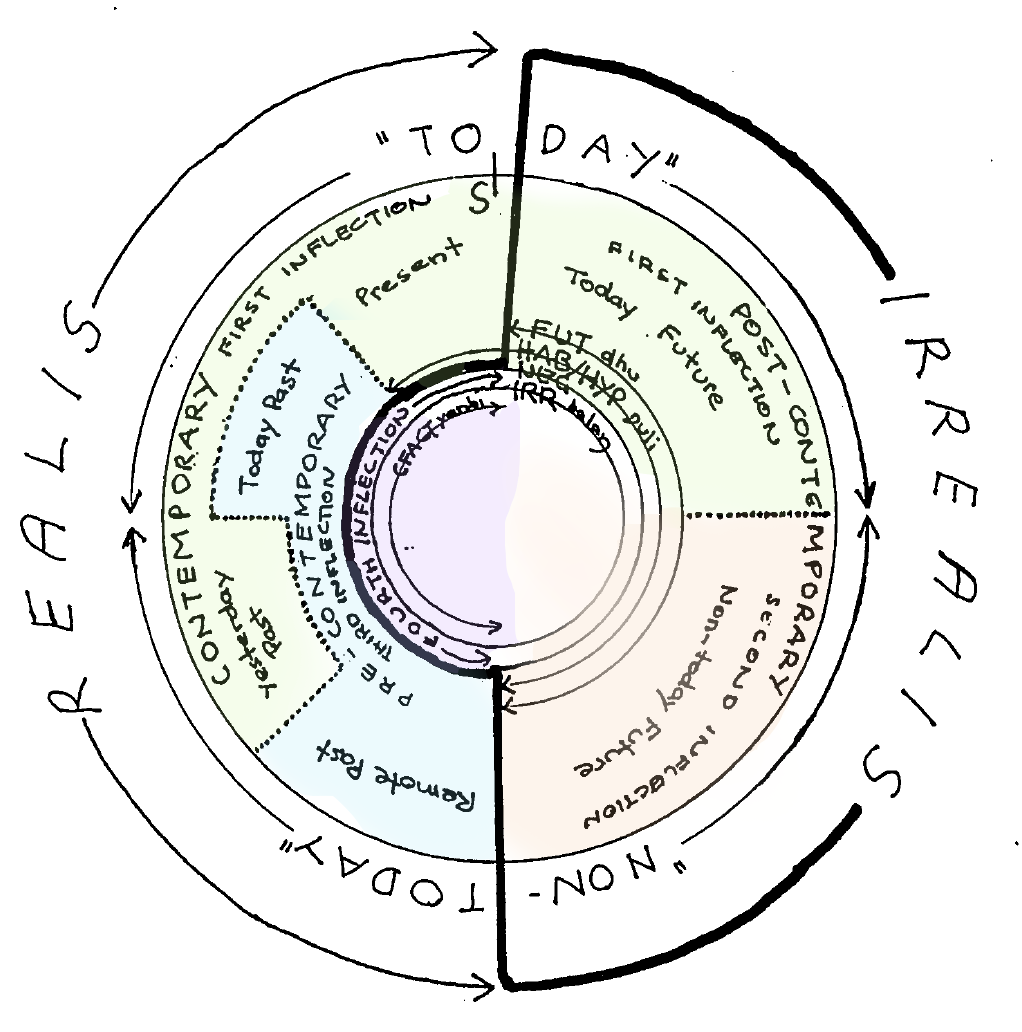
\includegraphics[width=0.75\textwidth]{WilkinsonDiagram362Col}
\end{figure}


\subsubsection{A division of labour.\\\textit{Inflectional morphology, auxiliaries and information structure}}

The work of encoding and interpreting temporal relations in Yolŋu discourse then cannot be explained without a theory of the interplay of semantics (of the verbal morphology and of auxiliaries) and pragmatics.

\paragraph{Verbal morphology: the semantics of inflection.} The data provided above, as summarised in the set of observations made of Dhuwal/Dhuwala that is given in table \ref{formdesc} above, allow us to make a series of immediate observations with respect to the relative contribution of the Yolŋu inflectional system for the encoding of temporal relations:
\begin{itemize}
	\item The subtlety of these categories, which appears to resist being understood as the encoding of a presupposition of pastness/presentness/futurity with respect to utterance time (\textit{i.e.} the `off-the-shelf' treatment of morphological tense);
	\item The (gradient) association of these inflectional categories with shades of modality/irreality;
	\item The complex association of tense as well as polarity, temporal aspect and perhaps speaker attitude with these modal categories.
\end{itemize}
\paragraph{the semantics of auxiliaries.} 
The interpretation of inflectional suffixes on the verb stem seems additionally to be substantially affected by the presence or absence of the various auxiliaries.

All four forms occur with \textit{ga+\textsc{infl}}$_{\texttt{[djr]}}$/\textit{gayŋa+\textsc{infl}}$_{\texttt{[dhg]}}$, the \textsc{ipfv} auxiliary, although the distributional restrictions on cooccurrence with other temporomodal particles (given in Table \ref{mods} below) is more complicated.

\begin{table}[h]
	\caption{Modal particles}\label{mods}\centering
\begin{tabular}{llll}



\textsc{\textbf{Particle}}&	\textbf{\begin{tabular}[c]{@{}c@{}}Wilkinson 1991\\ {\texttt{[djr]/[guf]}}\end{tabular}} & \textbf{\begin{tabular}[c]{@{}c@{}}McLellan 1992\\ \texttt{[dhg]}\end{tabular}}\\\midrule\midrule
\textbf{Future} & \textit{dhu} & \textit{barkthu} (?)\\\midrule
\textbf{Habitual}&\multirow{2}{*}{\textit{ŋuli}}&\textit{bayiŋ}\\
\textbf{Counterfactual}&&\textit{warri}\\\midrule
\textbf{Irrealis}&\textit{balaŋ}&\textit{ŋarru}

\end{tabular}\end{table}
McLellan describes the habitual, irrealis and realis ($\varnothing$) markers as existing in a ``paradigmatic relationship in a clause'' (1992:152), that is, all clauses are marked for one of these `modalities.' She goes on to investigate the apparent meanings of each by taking their basic meaning to be the contribution that each makes to a form I verb.

These modal particles have a range of effects on clausal interpretation that are briefly summarised in table \ref{formdesc} above; this provides an essential set of data for understanding the contributions made by each of these marking strategies to temporal and modal displacement. The fact that form III fails to tolerate any modal marking has been taken as evidence of its strict alignment with realis situations (e.g Wilkinson 1991:345; McLellan 1992: 164-5). 

Additionally, temporal particles/adverbials are used to provide information about the time span of a given event (examples listed in Table \ref{tempadv}). These particles all have clear distributional restrictions --- evidence of a strong correlation between inflectional form and temporal interpretation (\textit{e.g.} (\getfullref{pasts}a) above, see also Wilkinson 1991:341). Nevertheless, as was shown in (\getref{wangI}) above, particle selection is necessary for disambiguating past, present or future instantiation of the predicate with respect to utterance time.

\begin{table}[h]
	\caption{Temporal modification}\centering\label{tempadv}
\begin{tabular}{lll}
\textsc{\textbf{Particle}}&	\textbf{\begin{tabular}[c]{@{}c@{}}Wilkinson 1991\\ {\texttt{[djr]/[guf]}}\end{tabular}} & \textbf{\begin{tabular}[c]{@{}c@{}}McLellan 1992\\ \texttt{[dhg]}\end{tabular}}\\\midrule\midrule
\textbf{today} & gäthur		&\\
\textbf{now} & dhiyaŋ bala\\
\textbf{yesterday} & yawuŋgu/barpuru	&	yawungu/barpuru\\
\textbf{near future} & goḏarr'	&	barkthu\\
\textbf{future} &  boŋguŋ & \\
\textbf{`later'} & yalala & yalala\\
\textbf{distant past} & ŋäthil\\
\end{tabular}
\end{table}

The exact glosses of these adverbials are heuristic. Wilkinson points out that, while adverbial-like particles like \textit{boŋguŋ} and \textit{goḏarr} might both be glossable as `tomorrow' they can be used for ``any future event beginning with tomorrow.'' \textit{goḏarr} can only be used for roughly one post-crastinal week and can also refer to `morning', meaning it is also available for nonfuture contexts. She suggests, then, that a better semantics for \textit{goḏarr'} may be ``the early part of certain temporal domains'' (340), a description that may well have implicataions for our understanding of time reckoning in Yolŋu societies. Consequently, a treatment that builds vagueness into the semantics is highly informative in our goal of better understanding temporal perception and the interpretation of all of these lexical items.

An additional observation requiring further investigation is the relative infrequency of these particles in the small Ritharrŋu \texttt{[rit]} corpus provided in Heath 1980. Given the stronger apparent correlation between inflectional morphology and absolute time reference, a (very) preliminary hypothesis may be that the burden on these particles/auxiliaries is alleviated.

\paragraph{pragmatics: the role of context in discourse and information structure.}

Analogies between tense marking and pronouns have motivated a considerable amount of scholarship that has greatly informed the way we talk about the contribution of the tense morphology. In an influential 1973 article, Barbara Partee points to apparent deictic, anaphoric and `bound variable' uses of pronouns and tense markers (and potential constructions that lead to ambiguity between these uses.)   One of the most important insights of this work is an explicit move that shifts the burden of temporal interpretation to the context, both linguistically explicit and nonlinguistic.

Dynamic approaches to semantics and pragmatics attempt to better understand the role of information flow and conversational reasoning in properly accounting for these types of items. Certainly any treatment of metricality in tense marking seems to require reference to speaker perceptions of remoteness and specificity. Section \ref{lit} below outlines some of the tools and theoretical work available for understanding this interplay.

\section{Working at the intersection of temporal and modal semantics}\label{lit}
In the foregoing sections, we have seen examples of ways in which temporal and modal expression appear to interact and have inferred problems that these phenomena raise for our understanding of both of these categories. This section that follows comprises a compact overview of formal discussions of tense and tense-mood interactions (\textbf{§§\ref{intp}-\ref{ints}}), some examples of work on change in the temporal domain (§\textbf{\ref{dia}}), a synopsis of work on `tenselessness': how languages without morphological tense talk about time (\textbf{§\ref{tenseless}}), and a mention of (signs of a mounting interest in) investigation into the semantics of verbal inflection in Australian languages (\textbf{§\ref{aus}}).


In a 1998 paper, Angelika Kratzer extends Partee's discussion of the contextually determined properties of temporal interpretation and inflection to `sequence of tense' phenomena, explicitly referring to the `intimate ways' in which `[t]ense, aspect and modality interact...to fool us about their individual contribution[s] to the temporal semantics of sentences' (93). This is not a novel observation; it has long been observed that our theories of temporal expression are heavily  biased to discussions of dedicated tense (and to a lesser degree, aspect) given that these are the morphologised strategies on which Indo-European languages rely for temporal expression (e.g. Klein \& Li 2009:1; Klein 2009:41).



\subsection{Interpreting tense}\label{intp}


On \textit{p.}\pageref{yol-infl} above, I provided a brief discussion of one of the preponderant linguistic theories of tense. The presuppositional-indexical treament claims, in view of the reported deictic qualities of temporal reference, that the time of some event description is wholly contextually provided. Morphological tense marking, then, is basically a grammatical device which contains a presupposition that the runtime of the described event precedes, overlaps with, or follows speech time.

This referential treatment diverges somewhat from Priorian/Montogovian approaches which analyse tense operators as existential \textbf{quantifiers} over times, typed $\la\la i,t\ra,t\ra$. Following a quantificational semantics we, tense operator denotations are as ( below  (see \textit{e.g.} Dowty 1979:324).\footnote{A variant on this additionally lambda-binds the reference time ($\approx\boldsymbol{now}$), meaning a tense operator would be typed $\la i,\la\la i,t\ra,t\ra\ra$ (e.g. von Stechow 2009:140 or 1995:17 for a more complex version again.) Yolŋu Matha (\textit{sc.} the cyclic tense phenomenon generally) poses the same problems for this type of tense treatment.} \lingset{sampleexno=(ii)}
\pex\a$\denote{\textsc{pres}}^{g,c}=\lambda P\exists i.\boldsymbol{now}\sqsubseteq i\wedge P(i)$
\a$\denote{\textsc{pst}}^{g,c}=\lambda P\exists i.\boldsymbol{now}\succ i\wedge P(i)$
\a$\denote{\textsc{fut}}^{g,c}=\lambda P\exists i.\boldsymbol{now}\prec i\wedge P(i)$\xe


\subsection{Formalising tense and mood interaction}\label{ints}


The degree to which temporal readings `bleed into' markers that are traditionally associated with modality, and vice versa, is an area that has been attracting an increasing amount of scholarship in recent years, although these observations themselves are hardly new. Laca suggests that the the nonindependence of these two categories is primarily informed by the fact that `interpretation of modal verbs sometimes appears to be fully determined -- or at least severely restricted --- by the associated temporal configuration' (2008:1), providing the minimal pair in (\nextx) below as an example. Why is it that (a) receives an epistemic interpretation whereas (b) fails to admit of one?

\pex\a He must've left early\a He'll have to leave early\hfill(Laca 2008:1)\xe

Hacquard draws on similar data from French, where modal interpretation appears to be restricted by aspectual marking as in (\nextx) below. The (b) case appears to entail that an event of Jane taking the train actually occurred. This is not the case in (a).
\pex\a\begingl\gla Pour aller à Londres, Jane pouvait prendre le train//
\glb For go to London Jane can.\textsc{pst:ipfv.3s} take the train//
\endgl
\a\begingl\gla Pour aller à Londres, Jane put prendre le train//
\glb For go to London Jane can.\textsc{pst:pfv.3s} take the train//
\glft`To get to London, Jane could take the train'\hfill(Hacquard 2009: 283)//\endgl\xe


In an important 2002 article, Condoravdi considers the `temporal interpretation of modals', enriching the conceptualisation of modals by considering them a function from timelines\footnote{A \textit{timeline} might be defined as a temporal progression in a given world (i.e. state of affairs). This notion can be formalised by considering the Cartesian product of the set of worlds and set of times (viz. a set of $\la w,t\ra$ pairs.)} to propositions ${(f:\mathcal{W\times T\to\wp(W)})}$. This work has multiple important consequences, which I briefly outline here. 
\begin{enumerate}[label={\bf\roman*.}]
	\item The disentanglement of the temporal \textit{perspective} (time of access of the modal base) and temporal \textit{orientation} of a modalised assertion (the temporal relation between the temporal perspective and the time of the prejacent eventuality):
	\item Ambiguity between the counterfactual and epistemic readings of past-tensed modal statements (e.g. \textit{they might have won the game}) can now be accounted for by considering the relative scope relations of aspectual and modal operators (63\textit{ff}). \item Additionally, modals for the past can be understood as quantifying over `historical alternatives': sets of worlds that are identical at a particular point of evalution. These concepts and their consequences (e.g. `settledness') are essential tools in predicting the possible readings of \textit{bambai} as discussed in §\ref{rop} above.
	\item  Further, Condoravdi's analysis is accompanied by a pragmatically-driven principle (the `diversity condition') which predicts the infelicity of circumstantial readings of past-oriented modals.\footnote{Condoravdi's \textit{diversity condition} relates in an interesting way to the \textit{omniscience restriction} (6) proposed in the foregoing section on \textit{bambai.}}\end{enumerate}

Condoravdi's analysis has given rise to a current research program represented by recent work by Chen \textit{et al.} (2017) and Rullman \& Matthewson (to appear) among others, which considers the representation of past possibility and temporomodal interaction across typologically diverse languages. This work seeks to explain the interactions and apparent restrictions on all possible combinations of temporal orientation, perspective and modal base.

\iffalse\begin{itemize}
	\item Condoravdi 2002 (TMA stacking)
\item	von Fintel (and/or Kratzer) i.a. on the past-subjective stuff

\item Rullman \& Matthewson forthcoming `towards a theory of modal-temporal interaction'

\item Tonnhauser
\item Matthewson On the (non)future orientation of modals
\item Brenda \textsc{Laca} On modal tense and tensed modals  2008\textsc{ms}
\item Iatridou 2000 grammatical ingredients of counterf \textit{LI}
\item Hacquard 2006 PhD \textit{aspects of mod}
\item Eide 2003 Modals and Tense \textit{SuB}
\item Xling sems of tense mood mod (ed.	) \texttt{P294.5.C76X 200}
\item Arregui PhD dissertation \textit{acc of poss wolds: role of T and Asp}
\item Abusch Circ and temp dep in counterf modals \textit{NLS20}
\end{itemize}	\fi

	\subsection{Diachrony: temporal phenomena and meaning change}\label{dia}

The literature on grammaticalisation and semantic change provides many insights into the, primarily lexical, sources of TMA marking. Some of the best-known early surveys of these `pathways' include Bybee \textit{et al.}'s 1984 \textit{The Evolution of Grammar}, Hopper \& Traugott's 1993 \textit{Grammaticalization} and Traugott \& Dasher's 2002 \textit{Regularity in Semantic Change} (see Deo 2015a:180 for an appraisal of other work on the cross-linguistic meaning change similarities).

The phenomena described in the previous section, however have received nothing that resembles a functional treatment of the type that these grammaticalisation theorists have studied.\footnote{Note that Angelo \& Schultze-Berndt 2016 does include a short discussion of how mechanisms proposed by these theorists may be brought to bear on the emergence of apprehensional meaning in Kriol.}$^\text{,}$\footnote{The development of a rich metrical tense system in Kiksht is given some treatment in Silverstein (1974). The overarching thesis defended is that Chinookan languages to varying degrees `built' an entire morphosyntactic tense system out of the existence of a early Chinookan aspectual proclitic. He observes that ``corresponding to linear geographical extension from west to east, the ``tense'' category shows increasing development into an articulated morphosyntactic paradigm'' (S49). Kiksht in particular appears to have developed a particularly rich system of metrical tense that relies on deictic notions which Silverstein refers to as \textit{proximad} and \textit{distad} (S95). The nondurative past tense prefixes, for example, ``are elaborated to four...and the specifically temporal reference divides time before the speech event by specifying points before which the event predicated took place'' (S95). While Silverstein's thesis bears no direct relevance on the specific questions in this dissertation, methodologically, it represents an interesting example of the complete restructuring of an inflectional paradigm as understood through the comparison of the morphology of related languages.}
Comrie (1985) suggests that cyclic tense systems might be accorded `marginal status in the theory' given their cross-linguistic rarity, offering no insights into a possible synchronic analysis or diachronic trajectory.




\subsection{Integrating `tenseless languages' into the theory}\label{tenseless}

Discussed briefly in §\ref{cyctns}, languages that have been described as `tenseless' have posed a problem for our eurocentric theories of syntax and semantics. Here I briefly review a selection of recent, foregoing discussions of this problem as examples of treatments that these data have received.



Ritter \& Wiltschko (2009) for Halkomelem and Blackfoot , Matthewson (2006) for St'át'imcets, Tonhauser (2011) for Guaraní, Bohnemeyer (2009) for Yucatec and Bochnak (2016) for Washo all represent (a.o.) examples of discussions of the `problems' that underdocumented, ostensibly `tenseless' (or optionally tensed) languages, pose for existing theories of temporal expression. `Tenselessness' can be described as a property of a language for which ``topic times of utterances are not constrained vis-à-vis utterance times or reference points by the morphosyntactic form of the clause [excluding adverbial modification]''\footnote{Note that Bohnemeyer points out that speakers of so-called `tenseless languages' do not make significantly more frequent use of temporal adverbials than do speakers of tensed languages (2009:113).} (Bohnemeyer 2009: 85). 


 \textit{Contra} the basic \iffalse, mendacious \fi assumptions made in cartographic approaches adopted elsewhere in the syntactic literature (\textit{e.g.} Cinque \& Rizzi 2009:2), Ritter and Wilstchko's \textit{parametric substantiation hypothesis} (2009, 2014) suggests that the `substantive content' of a functional category \textsc{infl} (\textit{sc.} where tense marking is assumed to reside in most Indo-European languages) varies cross-linguistically. They propose that different languages may variably also associate this projection with spatial (\textit{e.g.} Halkomelem \texttt{[hur]} Salishan: Pacific Northwest) or participant marking (\textit{e.g.} Blackfoot \texttt{[bla]} Algonquian: Alberta). This type of analysis seeks to account for the optionality or absence of tense morphology across languages, characterising \textsc{infl} more broadly as a projection that houses some \textit{deictic category}, serving to anchor the reported event to an utterance (2009:193).%\mcom{challenging scholarship that intimately/causally/unidirectionally relates syntax (notions of finiteness) and semantics (notions of tense marking etc)}


		%    

Matthewson (2006) posits the existence of a covert, obligatory morpheme in arguing for the existence of a future/nonfuture distinction in St'át'imcets (\texttt{[lil]} Algonquian: British Columbia) \textit{i.e.} she claims that this language's tenselessness is illusory). The denotation given for this covert nonfuture item is of the indexical type discussed above. St'át'imcets does however contain a number of lexical items (a clitic, an auxiliary and a number of other periphrastic constructions) which must be used in order to express the future. Matthewson provides a detailed argument for the treatment of clitic \textit{kelh} as a temporal marker with a semantics similar to that of Abusch (1985)'s \textsc{\textit{woll}}.

 

Conversely, Bohnemeyer (2009) makes use of the notion of `temporal anaphora' --- effectively a discourse structuring principle and one that is operationalised elsewhere in dynamic semantic frameworks (\textit{e.g.} DRT in Partee 1984, Roberts 1989) --- in accounting for the temporal interpretation of sentences in Yucatec (\texttt{[yua]} Mayan: Yucatán). Further building on this treatment, Tonhauser (2011) also explicitly eschews appeal to covert tense in her treatment of Paraguayan Guaraní \texttt{[gug]} despite the latter's apparent similarity to St'át'imcets (268). She instead couches her analysis in a dynamic semantics that seeks to formalise the flow of information through discourse, taking the meaning of a given utterance to be its context change potential. 


\subsection{The semantics landscape in Australia} \label{aus}
As discussed above, Australia's 400+ languages have been extremely under-represented in the elaboration of formal semantic theory. As a consequence of this, existing descriptions of these, particularly with respect to categories like tense, modality and aspect, do not integrate obviously with the assumptions made in much of the literature.

Exceptions to this include a 2012 themed issue of the \textit{Australian Journal of Linguistics}, which emerged out of an explicit project to ``bring together the grammatical description and typological investigation of Australian languages with the formal semantic investigation of tense, aspect, mood and evidentiality, in the understanding that these areas have much to offer one another' (see Stirling \& Dench 2012:1).\footnote{The spirit of this project has also given rise to a Australia-Pacific TAM marking workshop to take place at the Australian Linguistic Society meeting this December.} As has hopefully been made clear in this prospectus, I agree with Sterling \& Dench on this latter count.

\section{Proposal: dissertation structure}
\subsection{A chapter outline}
\textbf{Chapter 0.} \textsc{Introduction} to research question.
\begin{description}[labelindent=.8cm]


\item[Chapter 1.] \textsc{The language ecology}: Geolinguistic, anthropological and sociohistorical background to Arnhem land.
\item[Chapter 2.] \textsc{General literature:} An overview of the logics of tense and modality and linguistic approaches to these categories. Discussion of previous scholarship on the interdependence of tense, mood and aspectual interpretation.
\end{description}
\textbf{\textsc{Part I.}} \textsc{The Kriol modal domain and emergence of apprehensionality}
%this one word can teach us this about this and how this happens. dia, 
%let's look at the dia stuff, this can help us understand pt 2... <<<guides solutions, possible answers etc. how temp<>modal >>> meaning
\begin{description}[labelindent=.8cm]


\item[Chapter 3.] \textsc{Data}: Background of the verbal inflection domain in Australian Kriol.\\\textit{bambai:} how has a temporal frame adverbial become complicit in encoding modal meaning?
\item[Chapter 4.] \textsc{A formal analysis of \textit{bambai} polysemy}\\Speaker meaning, information structure and restricting the domain of quantification.\\Implications for understanding other `discourse anaphors' (e.g. \textit{other(wise)})
\item[Chapter 5. ] \textsc{Diachronic insights:} How can we understand the emergence of apprehensional readings for \textit{bambai}?\\Does a theory of this process (and the synchronic analysis more broadly) provide evidence of shared conceptual resources for interpreting futurity and epistemic modalities?
\end{description}
\textbf{\textsc{Part II.}} \textsc{Comparative Yolŋu: restructuring of the verbal-inflectional paradigm and the expression of time}
%let's look at the entire inflectional system of one language and borrow insights from what we learned in pt 1.
\begin{description}[labelindent=.8cm]
\item[Chapter 6. ]\textsc{Data:} A thorough comparative description of the semantics of verbal paradigms across multiple Yolŋu varieties.\\Field-informed discussion of strategies for expressing temporal and modal relations in Gupapuyŋu and Ritharrŋu.
\item[Chapter 7. ] \textsc{A formal account of TMA marking in Yolŋu}
\item[Chapter 8. ] \textsc{A diachronic dimension:} Likely contact-induced meaning change in the TMA paradigms.
\end{description}
\textbf{Chapter 9.} \textsc{Theoretical contribution} and envoi.

\subsection{$\boldsymbol{\langle \mathcal{T},\mathcal{I},\prec,\sqsubseteq,\mathcal{Q},t\!*\rangle}$}
\centering
\begin{tabular}{cl}
	$\boldsymbol{i\in\mathcal{I}}$ & \multicolumn{1}{c}{$\boldsymbol{e\in\mathcal{E}}$}\\\toprule\toprule
	\textsc{\textbf{til End 2017}} & A dynamic semantic (\textsc{Ch. 4}) account of \textit{otherwise}\\\midrule %fplanning, drafting of structures for chapters relying on nuanced discussion of existing theory, literature, revision of bambai (chs 1-4), rev 3,5, comp of data for 6 (structuring elicitation plan). 6-8 fall into spring, 9 in late spring. Aiming for may/june submission. File.
	\textsc{\textbf{Winter 2018}} & \begin{tabular}{l}
		• Grant applications (fieldwork)\\
		• Field planning\\
		• Two handbook chapters\\
	\end{tabular}\\\midrule
	\textbf{\textsc{Spring 2018}} & \begin{tabular}{l}
		• Complete \textsc{\textbf{Part I}} draft\\\hspace*{.5cm}(information-structural account of \textit{bambai})\\
		• Field planning
	\end{tabular}\\\hline
	\textsc{\textbf{Summer 2018}} &\begin{tabular}{l} • Fieldwork (Gapuwiyak/Galiwin'ku \& Ngukurr)\\
	• Begin \textsc{Chapter 6}\end{tabular}\\\midrule
\textsc{\textbf{Autumn 2018}} & Complete \textsc{\textbf{Part II}} draft\\\midrule
\textbf{\textsc{Winter 2019}} & Write \textsc{chapter 9}\\\midrule
\textbf{\textsc{Spring 2019}} & \begin{tabular}{l}
	• Compile dissertation\\
	• Review all chapters\\
	• Defend dissertation\\
	• Submit dissertation\\
	• Get a job\\
	• Graduate\\
%	• Win lottery\\
\end{tabular}\\\bottomrule
\end{tabular}

\justifying
%\subsection{Parting words: potential contributions} Merged into intro§1


\setcounter{secnumdepth}{0} 
\vfill\section{Bibliography}%\mcom{incomplete, i gave up on Bib\TeX for the timebeing so am compiling manually now.}
\subsection{Works cited}

\small\begin{hangparas}{3em}{1}

Abusch, D. (1985). \textit{On verbs and time}. [PhD dissertation], University of Massachussetts, Amherst.   


Angelo, D., \& Schultze-Berndt, E. (2016). Beware bambai – soon it may turn apprehensive. In F. Meakins \& C. O'Shannessy (Eds.), \textit{Loss and Renewal: Australian languages since contact} (pp. 255-296). Berlin: Mouton de Gruyter.

Bochnak, M. R. (2016). Past time reference in a language with optional tense. \textit{Linguistics \& Philosophy, 39}(4), 247-294. 

Bohnemeyer, J. (2009). Temporal anaphora in a tenseless language: the case of Yucatec. In W. Klein \& P. Li (Eds.).


Chen, S., Hohaus, V., Laturnus, R., Louie, M., Matthewson, L., Rullmann, H., . . . Vander Klok, J. (2017). Past possibility cross-linguistically: Evidence from 12 languages. In A. Arregui, M.-L. Rivero, \& A. Salanova (Eds.),\textit{ Modality Across Syntactic Categories}. Oxford: OUP.


Comrie, B. (1985). \textit{Tense}. Cambridge: Cambridge University Press.



Condoravdi, C. (2002). Temporal Interpretation of Modals: Modals for the Present and for the Past. In L. Casillas, B. Clark, \& S. Kaufmann (Eds.), \textit{The construction of meaning}. Stanford: CSLI publications.


Copley, B. L. (2002). \textit{The Semantics of the Future}. (PhD dissertation), MIT, Cambridge, MA.   

Deo, A. (2006). \textit{Tense and Aspect in Indo-Aryan Languages: Variation and diachrony.} (PhD dissertation), Stanford University, Stanford, CA.   

---. (2015a). Diachronic Semantics.\textit{ Annual Review of Linguistics, 1,} 179-197. 

---. (2015b) The semantic and pragmatic underpinnings of grammaticalization paths: The progressive to imperfective shift.\textit{ Semantics and Pragmatics, 8}(14), 1-52. 


Dickson, G. (2015). \textit{Marra and Kriol: the loss and maintenance of knowledge across an language shift boundary.} (PhD thesis), Australian National University, Canberra.   

Dowty, D. (1979).\textit{ Word Meaning and Montague Grammar.} Dordrecht: Kluwer.



Eckardt, R. (2006).\textit{ Meaning Change in Grammaticalization: An enquiry into semantic reanalysis}. Oxford: OUP.


Glasgow, K. (1964). \textit{Frame of reference for two Burera tenses.} \textsl{non vidi.}


Hacquard, V. (2009). On the interaction of aspect and modal auxiliaries. \textit{Linguistics and Philosophy, 32}(3), 279-315. 


Harris, J. (1986). Northern Territory Pidgins and the Origin of Kriol. In S. A. Wurm (Series Ed.) Canberra, \textit{Pacific Linguistics.}


Heim, I. R. (2011[1982]). \textit{The semantics of definite and indefinite noun phrases.} (PhD dissertation), University of Massachusetts, Amherst.   



Hockett, C. F. (1960). The Origin of Speech. \textit{Scientific American, 203}(3), 88-97. 

Horton, D. R. (Cartographer). (1996). Aboriginal Australia Wall Map. AIATSIS, Canberra, ACT.



Kamp, H. (1981). A theory of truth and semantic representation In J. Groenendijk, T. Janssen, \& M. Stokhof (Eds.),\textit{ Formal Methods in the Study of Language, Part I}. Amsterdam: Mathematsich Centrum.



Klein, W. (2009). How time is encoded. In W. Klein \& P. Li (Eds.).


Klein, W., \& Li, P. (Eds.). (2009).\textit{ The Expression of Time}. Berlin; New York: Mouton de Gruyter.



Kratzer, A. (1981). The Notional Category of Modality. In H.-J. Eikmeyer \& H. Rieser (Eds.),\textit{ Words, worlds, and contexts: New Approaches in Word Semantics }(pp. 38-74). Berlin; NY: Walter de Gruyter.


---. (1998). More Structural Analogies Between Pronouns and Tenses. Paper presented at Semantics and Linguistic Theory \textbf{VIII}, Ithaca. \url{https://journals.linguisticsociety.org/proceedings/index.php/SALT/article/view/2808}



---. (2012).\textit{ Modals and Conditionals}. Oxford: OUP.


Hopper, P. J., \& Traugott, E. C. (1993). \textit{Grammaticalization}. Cambridge: Cambridge University Press.


Laca, B. (2012).\textit{ On modal tenses and tensed modals. }Ms.


Lichtenberk, F. (1995). Apprehensional Epistemics. In J. Bybee \& S. Fleischman (Eds.), \textit{Modality in Grammar and Discourse.} Amsterdam: John Benjamins.

Lowe, B. M. (1996). \textit{Grammar Lessons in Gupapuyŋu} (M. Christie Ed.). Darwin, NT: Yolŋu Studies, CDU.


Matthewson, L. (2006). Temporal semantics in a superficially tenseless language.\textit{ Linguistics \& Philosophy, 29}(6), 673-713. 

McLellan, M. (1992).\textit{ A Study of the Wangurri Language.} (PhD thesis), Macquarie University, Sydney.   


Palffy-Muhoray, N. (2016).\textit{ Hungarian Temporal and Aspectual Reference in the Absence of Dedicated Markers.} (PhD Dissertation), Yale University, New Haven, CT.   

Partee, B. H. (1973). Some Structural Analogies between Tenses and Pronouns in English. \textit{The Journal of Philosophy, 70}(18), 601-609. \texttt{doi:10.2307/2025024}

---. (1984). Nominal and temporal anaphora. \textit{Linguistics \& Philosophy, 7}(3), 243-281. 


Ritter, E., \& Wiltschko, M. (2009). Varieties of INFL: Tense, location and person. In J. Van Craenenbroeck (Ed.), \textit{Alternatives to cartography} (pp. 153-202). Berlin; New York: Mouton de Gruyter.

---. (2014). The composition of INFL: An exploration of tense, tenseless languages, and tenseless constructions. \textit{Natural Language \& Linguistic Theory, 32}, 1331-1386. 




Roberts, C. (1989). Modal Subordination and Pronominal Anaphora in Discourse. \textit{Linguistics \& Philosophy, 12}(6), 683-721. 


---. (1998). Focus, the flow of information and universal grammar. \textit{Syntax and Semantics, 29}, 109-160. 


Rullmann, H., \& Matthewson, L. (to appear). Towards A Theory of Modal-Temporal Interaction. \textit{Language}. 

Sandefur, J. R. (1986).\textit{ Kriol of North Australia: a language coming of age}. Darwin: SIL-AAB.

Silverstein, M. (1974). Dialectal developments in Chinookan tense-aspect systems: an areal-historical analysis. \textit{International Journal of American Linguistics, 40}(4.2), S49-S99. 


Stalnaker, R. (1979). Assertion. In P. Cole (Ed.), \textit{Syntax and Semantics}. New York: Academic Press.

von Stechow, A. (1995). On the proper treatment of tense. Paper presented at \textit{Semantics and Linguistic Theory V}, Ithaca, NY. 


---. (2009). Tenses in compositional semantics. In W. Klein \& P. Li (Eds.) (pp. 129-166). 

Stirling, L., \& Dench, A. (2012). Tense Aspect Modality and Evidentiality in Australian Languages: Foreword.\textit{ Australian Journal of Linguistics, 32}(1), 1-6. 

Tonhauser, J. (2011). Temporal reference in Paraguayan Guaraní: a tenseless language. \textit{Linguistics \& Philosophy, 34}(3), 257-303. 

Traugott, E. C., \& Dasher, R. B. (2002). \textit{Regularity in Semantic Change.} Cambridge, UK: Cambridge University Press.


Wilkinson, M. P. (1991). \textit{Djambarrpuyŋu: a Yolŋu variety of Northern Australia.} (PhD thesis), University of Sydney, NSW.   


\end{hangparas}\vspace*{.75in}

\subsection{Further reading}\begin{hangparas}{3em}{1}


Caudal, P., Dench, A., \& Roussarie, L. (2012). A Semantic Type-driven Account of Verb-formation Patterns in Panyjima.\textit{ Australian Journal of Linguistics, 32}(1), 115-155. 

Eather, B. (2011/2017).\textit{ A grammar of Nakkara (Central Arnhem Land coast).} Munich: Lincom.


Green, R. (1987).\textit{ A sketch grammar of Burarra. [Hons thesis]}, ANU, Canberra, ACT.   


---. (1995). \textit{Gurr-goni (North Central Arnhem Land)}. [PhD thesis], ANU, Canberra, ACT.   



Hohaus, V. (submitted). \textit{Counterfactuality and Past. }

Hyman, L. M. (1980). Relative time reference in the Bamileke tense system. \textit{Studies in African Linguistics, 11}(2), 227-237. 



Martin, J. B. (2010). How to Tell a Creek Story in Five Past Tenses. \textit{International Journal of American Linguistics, 76}(1), 43-70. \texttt{doi: 10.1086/652754}





Matthewson, L. (2010). Cross-linguistic variation in modality systems: The role of mood. \textit{Semantics and Pragmatics, 3}(9), 1-74. 


Nordlinger, R., \& Caudal, P. (2012). The Tense Aspect and Modality System in Murrinh-Patha. \textit{Australian Journal of Linguistics, 32}(1), 73-113. 

Nordlinger, R. \& Sadler, L. (2008). When is a temporal marker not a tense?: Reply to Tonhauser 2007. \textit{Language, 84}(2), 325-331. 



Ritz, M.-E., Dench, A., \& Caudal, P. (2012). Now or Then? The Clitic -rru in Panyjima: Temporal Properties in Discourse.\textit{ Australian Journal of Linguistics, 32}(1), 41-72. 


Schultze-Berndt, E. (2012). Pluractional Posing as Progressive: A construction between Lexical and Grammatical Aspect.\textit{ Australian Journal of Linguistics, 32}(1), 7-39. 

Smith, C. S., Perkins, E. T., \& Fernald, T. B. (2007). Time in Navajo: Direct and Indirect Interpretation. \textit{International Journal of American Linguistics, 73}(1), 40-71. 


Stirling, L. (2012). Tense Aspect Shifting in Kala Lagaw Ya Oral Narratives. \textit{Australian Journal of Linguistics, 32}(1), 157-190. 


--- \& Dench, A. (2012). Tense Aspect Modality and Evidentiality in Australian Languages: Foreword. \textit{Australian Journal of Linguistics, 32}(1), 1-6. 

Stone, M., \& Hardt, D. (1999). Dynamic Discourse Referents for Tense and Modals. In H. Bunt \& R. Muskens (Eds.), \textit{Computing Meaning: Volume 1} (pp. 301-319). Dordrecht: Springer Netherlands.


Tonhauser, J. (2007). Nominal Tense? The meaning of Guaraní nominal temporal markers. \textit{Language, 83}(4), 831-869. 


Tonhauser, J. (2011). Temporal reference in Paraguayan Guaraní: a tenseless language. \textit{Linguistics \& Philosophy, 34}(3), 257-303. 

Tonhauser, J. (2015). Cross-Linguistic Temporal Reference. \textit{Annual Review of Linguistics, 1,} 129-154. 


van der Wal, A. E. (1992). \textit{Structure and Function in Gupapuyŋu: a Yolŋu dialect of North-east Arnhemland.} (PhD thesis), University of Newcastle, NSW.   


Verstraete, J.-C. (2006). The Nature of Irreality in the Past Domain: Evidence from Past Intentional Constructions in Australian Languages. \textit{Australian Journal of Linguistics, 26}(1), 59-79. \texttt{doi: 10.1080/07268600500531636}




\end{hangparas}
\setcounter{secnumdepth}{2} \newpage\appendix
\section{\textit{Yolŋu data}}
\textit{Except where noted, the data that follows and the page numbers cited are drawn from Wilkinson (1991) on Djambarrpuyŋu \texttt{[djr]}. These data provide an overview of the categorised functions of each inflection, enumerated in Table \ref{formdesc} on page \pageref{formdesc} of this document.}
\small
\subsection{primary inflection (I)}
\pex\begingl\deftagex{prI}
\glpreamble\textsc{Present}//
\gla ŋarra \textbf{marrtji}-n dhiyaŋu-n bala//
\glb 1s go.\textbf{I}-\textsc{seq} \textsc{prox.erg-seq} away//
\glft`I am going now'\hfill(256)//
\endgl\xe

\pex\begingl\deftagex{pstI}
\glpreamble\textsc{Past}//
\gla yo, barpuru-ny ŋarra ŋanya nhä-\textbf{ma}-ny//
\glb yes yesterday\textsc{-prom} 1s 3s.\textsc{acc} see-\textbf{I}-\textsc{prom}//
\glft`yeah, I saw him yesterday'\hfill(339)//
\endgl\xe

\pex\a\begingl\deftagex{habI}
\glpreamble\textsc{present habitual}//
\gla ŋunhi ŋilinyu \textbf{ŋuli} ga warkthu-\textbf{n} maṉḏa waŋgany-ŋur//
\glb \textsc{texd} 1d\textsc{.incl} \textsc{\textbf{hab}} \textsc{ipfv.\textbf{I}} work-\textbf{I} 3d one-\textsc{loc}//
\glft`us two, who are working in the one work'\hfill(348)//\endgl
\a\begingl\glpreamble\textsc{Past habitual}//
\gla ŋarra \textbf{ŋuli} ga rur'yun munhawumirri yan bitjan~bili//
\glb 1s \textsc{\textbf{hab}} \textsc{ipfv.\textbf{I}}//
\glft `I always get up early in the morning'\hfill(348)//
\endgl\xe

\pex\begingl\deftagex{futI}\glpreamble \textsc{today Future}//
\gla yalala ŋarra dhu nhokal lakara-\textbf{m}//
\glb later 1s \textsc{fut} 2s.\textsc{obl} tell-\textbf{I}//
\glft`I'll tell you later (today)'\hfill(346)//\endgl\xe

\pex \textsc{Cooccurrence with \textit{ŋuli}}
\a\begingl\glpreamble\textsc{Present habitual}//
\gla ŋarra \textbf{ŋuli} ga rur'yun munhawumirri yan bitjan~bili//
\glb 1s \textsc{\textbf{hab}} \textsc{ipfv.\textbf{I}} get\_up.\textbf{I} early~morning \textsc{emp} always//
\glft`I always get up early in the morning'\hfill(348)//\endgl
\a\begingl\glpreamble\textsc{Hypothetical (conditional) use}//
\gla \textbf{ŋuli} nhe dhu warku'yu-\textbf{n} wuŋgan-nha, nayi-ny \textbf{dhu} läwu-\textbf{m}//
\glb \textsc{\textbf{hyp}} 2s \textsc{fut} annoy-\textbf{I} dog\textsc{-acc} 3s-\textsc{prom} \textsc{fut} bite\textbf{-I}//
\glft `if you tease the dog, it'll bite'\hfill(350)//
\endgl\xe

\subsection{secondary inflection (II)}
\pex\deftagex{imprII}\begingl\glpreamble\textsc{Imperative}//
\gla yaka \textbf{waŋi}!//
\glb \textsc{neg} talk.\textbf{II}//
\glft`don't speak!'\hfill(360)//\endgl\xe

\pex\textsc{Future}\deftagex{futII}
\a\begingl\glpreamble\textsc{without \textit{dhu}}//
\gla ŋayi boŋguŋ \textbf{nhini} \textbf{ŋäku} ŋarra-ny ŋunhal yirrkala//
\glb 1s tomorrow sit.\textbf{II} hear;\textbf{II} 1s\textsc{-acc} \textsc{dist.loc} \textsc{name}//
\glft`They will be there at Yirrkala listening to me (in several weeks' time)'\hfill(340)//
\endgl
\a\begingl\glpreamble\textsc{with \textit{dhu}}//
\gla goḏarr'nha ŋarra dhu nhuŋu dhäwu-ny lakara-\textbf{ŋ}//
\glb tomorrow\textsc{-seq} 1s \textsc{fut} 2s\textsc{.dat} story\textsc{-prom} tell-\textbf{II}//
\glft`I'll tell you the story tomorrow'\hfill(346)//\endgl
\a\begingl\gla yalala-ŋu-mirri-y ŋula~nhätha ŋarra dhu nhokal lakara-\textbf{ŋ}//
\glb later-ŋu\textsc{-prop-erg} sometime 1s \textsc{fut} 2s\textsc{.obl} tell-\textbf{II}//
\glft`I'll tell you the story tomorrow'\hfill(346)//\endgl\xe

\pex \textsc{Cooccurrence with \textit{ŋuli}}\\
\a\begingl\glpreamble\textsc{Future habitual}\hfill\textit{note here that there's a strong hypothetical flavour in this datum}//
\gla nhä-mirr \textbf{balaŋ} ŋayi gi ŋirrimbu-\textbf{ŋ} ŋarra-kal milmitjpa-ny ga goḏarr'-tja ŋayi \textbf{ŋuli} gi dhiyal warkthu-\textbf{rr}//
\glb what-\textsc{prom} \textsc{irr} 3s \textsc{ipfv.\textbf{II}} come-\textbf{II} 1s-\textsc{obl} afternoon\textsc{-prom} and morning\textsc{-prom} 3s \textsc{\textbf{hab}} \textsc{ipfv.\textbf{II}} \textsc{prox-loc} work\textbf{-II}//
\glft`How about she come to me in the afternoon and works here in the morning?'\hfill(351)//
\endgl
\a\begingl\glpreamble\textsc{Hypothetical (conditional) use}\hfill\textit{appears to be less frequent than with \textbf{I} for indicatives}//
\gla \textbf{ŋuli} ŋayi dhu dhuwal raki djaw'yu-\textbf{rr}-nydja boŋguŋ Melanie-y dhäruk-mirr ŋarr-kalaŋu-mirr-nydja bala ŋayi dhu gi bäki-n nhakun nhanukiyin-galalaŋu-wurr ŋä-nha-kurr//
\glb \textsc{hyp} 3s \textsc{fut} \textsc{prox} tape take-\textbf{II}-\textsc{prom} tomorrow \textsc{name-erg} word\textsc{-prop} 1s\textsc{-obl-prop-prom} then 3s \textsc{fut} \textsc{ipfv.\textbf{II}} use\textsc{-seq} like 3s\textsc{.emph-obl-perl} listen\textsc{-\textbf{IV}-perl}//
\glft`If they take this tape, then later Melanie will be using it, perhaps by listening (to it)'\hfill(352)//\endgl
\xe

\pex\begingl\deftagex{negII}\glpreamble \textsc{Negative recent past}//
\gla bäyŋu ŋayi gi \textbf{nhini} barpuru//
\glb \textsc{neg} 3s \textsc{ipfv.\textbf{II}} sit.\textbf{II} yesterday//
\glft`They weren't staying here yesterday'\hfill(357)//\endgl\xe

\pex\textsc{Cooccurrence with explicit modal \textit{balaŋ} `IRR'}
\a\begingl
\gla ŋayi balaŋ limurruŋ maḏakarritj-thi//
\glb3s \textsc{irr} 1d\textsc{.incl-dat} angry\textsc{-inch.\textbf{II}}//
\glft`she may be angry with us (today)'\hfill(354)//
\endgl
\xe
\subsection{tertiary inflection (III)}
\pex\textsc{Past}\deftagex{pstIII}
\a\deftaglabel{today}\begingl\glpreamble\textsc{today}//
\gla ŋe gaathur ŋarra ŋaɲa nhaa-\textbf{ŋal} goḏarr dhiyal//
\glb	yes, today 1s 3s{\sc.acc} see-\textbf{III} morning {\sc prox-loc}//
\glft`Yes, I saw him here this morning'\hfill(339)//\endgl
\a\deftaglabel{dist}\begingl\glpreamble\textsc{distant/non-specific}//
\gla maarrma ga-\textbf{n} malwan-dja dhaara-\textbf{n} yindi maṉḏa-ɲ//
\glb two {\sc ipfv-\textbf{III}} Hibiscus-{\sc prom} stand-\textbf{III} big 3d-{\sc prom}//
\glft`Two big Hibiscus flowers were growing there' (at some place in the speaker's youth)//\hfill(339)
\endgl\xe


\pex\textsc{$\Psi$ uses}


%`The description of such states rel. to the moment of speech appears to invoke a general temporariness to the state. it is quite poss with a pred such as \textit{rirrikthu-N} `be sick, in pain' for sb to be seen as in that state for a long period of time. Then \textbf{III} is not required. the use of\textbf{ I} in this context however would appear to be relative to `nowadays' rather than the actual moment of speech... perfective.' (\textbf{I}  cooccurs with \textit{gana} to reduce affectedness.)

\a\begingl\gla ŋarra dhuwal/dhika djawaryu-\textbf{rr}/rerrikthu-\textbf{rr}/djanŋarrthi-\textbf{n}//
\glb 1s \textsc{prox/indefp} be.tired-\textbf{III}/be.sick-\textbf{III}/be.hungry-\textbf{III}//
\glft`I'm (a bit) tired/sick/hungry'\hfill(278)//\endgl
\a\begingl\gla bili djawar'yu-\textbf{rr}-a//
\glb \textsc{complv} be.tired-III//
\glft`They're already tired'\hfill(365)//\endgl
\xe
\subsection{quarternary inflection (IV)}
\pex\deftagex{nuliIV}\textsc{Cooccurrences with \textit{ŋuli} `hyp/hab'}\a\begingl\glpreamble\textsc{Past habitual}\deftaglabel{hab}//
\gla ga ŋayi-ny \textbf{ŋuli} yarrupthu-\textbf{na}-n ganybu-lil-a dharpu-\textbf{nha}-lil ga linyu-ny \textbf{ŋuli} ḏuwatthu-na-n...//
\glb  and 3s-\textsc{foc} \textsc{hab} go.down-\textbf{IV}-\textsc{seq} net\textsc{-all-seq} sew-IV\textsc{-all} and 2d\textsc{.incl.foc} \textsc{hab} go.up-\textbf{IV}\textsc{-seq}//
\glft`And then she  would go and sew fishing nets and we two  would go up...'\hfill(350)//
\endgl
\a\deftaglabel{hyp}\begingl\glpreamble\textsc{`Hypothetical' (counterfactual)}//
\gla ŋäthil ŋarra \textbf{ŋuli} \textbf{balaŋ} ḻiya-ŋamaŋamayu-n-mi-\textbf{nya} bala ŋarra \textbf{balaŋ} waŋa-nha-n//
\glb earlier 1s \textsc{hyp} \textsc{irr} have.idea-1-\textsc{r/r}-\textbf{IV} then 1s \textsc{irr} speak-\textbf{IV}-\textsc{seq}//
\glft`Had I thought of it before, I would've spoken'//
\endgl\xe
\pex[]<biv> \textsc{Cooccurrence with \textit{balaŋ} `irr'}
\a\begingl
\gla barpuru \textbf{balaŋ} ŋarra bala dentist-kal marrtji-\textbf{nya} dhiyak filling-gu//
\glb yesterday \textsc{\textbf{irr}} 1s \textsc{away} dentist-\textsc{obl} go-\textbf{IV} \textsc{prox.dat} filling\textsc{-dat}//
\glft`yesterday I should have gone to the dentist for a filling'\hfill(353)//
\endgl
\a\begingl
\gla märr \textbf{balaŋ} ŋayi yaka dharpa-ny galkirri-nya be-ŋur-nydja garramat-ŋur-nydja//
\glb such.that \textsc{\textbf{irr}} 3s \textsc{neg} tree-\textsc{foc} fall-\textbf{IV} \textsc{indef-abl-foc} top-\textsc{abl-foc}//
\glft`(she drove slowly) so the tree wouldn't fall off the top'\hfill(354)//
\endgl
\xe
\pex\textsc{Remote past under negation}\\
\begingl\gla ŋäthil-nydja ŋarra ga-\textbf{n} dhuwal, ga miltjirri marrtji-\textbf{n} bäyŋu ŋarra ŋuli ga-nha nhä-\textbf{nha}	//
\glb before\textsc{-prom} 1s \textsc{ipfv-\textbf{III}} \textsc{prox} and blind go\textsc{-\textbf{III}} \textsc{neg} 1s \textsc{hab} \textsc{ipfv-IV} see-\textbf{IV}	//
	\glft`I was blind before, I wasn't able to see'\hfill(358)//
\endgl\xe
\vfill\setcounter{secnumdepth}{0}\section{List of abbreviations}
\footnotesize\begin{tabular}{ll}
	\textsc{acc}	&	accusative\\
	\textsc{all}	&	allative\\
	\textsc{complv}	&	completive\\
	\textsc{dat}	&	dative\\
	\textsc{emp}	&	emphatic\\
	\textsc{erg}	&	ergative\\
	\textsc{hab}	&	habitual\\
	\textsc{hyp}	&	hypothetic\\
	\textsc{incl}	&	inclusive\\
	\textsc{ipfv}	&	imperfective\\
	\textsc{irr}	&	irrealis\\
	\textsc{loc}	&	locative\\
	\textsc{mod}	&	modal\\
	\textsc{neg}	&	negative\\
	\textsc{obl}	&	oblique\\
	\textsc{perl}	&	perlative\\
	\textsc{prom}	&	prominent\\
	\textsc{prox}	&	proximate\\
	\textsc{pst}	&	past\\
	\textsc{red}	&	reduplicant\\
	\textsc{seq}	&	sequential\\
	\textsc{texd}	&	text-deictic\\
	\textsc{tr}	&	transitive\\
	
\end{tabular}
\end{document}